\clearpage
\setcounter{page}{1}

\twocolumn[{
\renewcommand\twocolumn[1][]{#1}

\maketitlesupplementary
\begin{center}
  \centering
  % \vspace{-0.2in}
    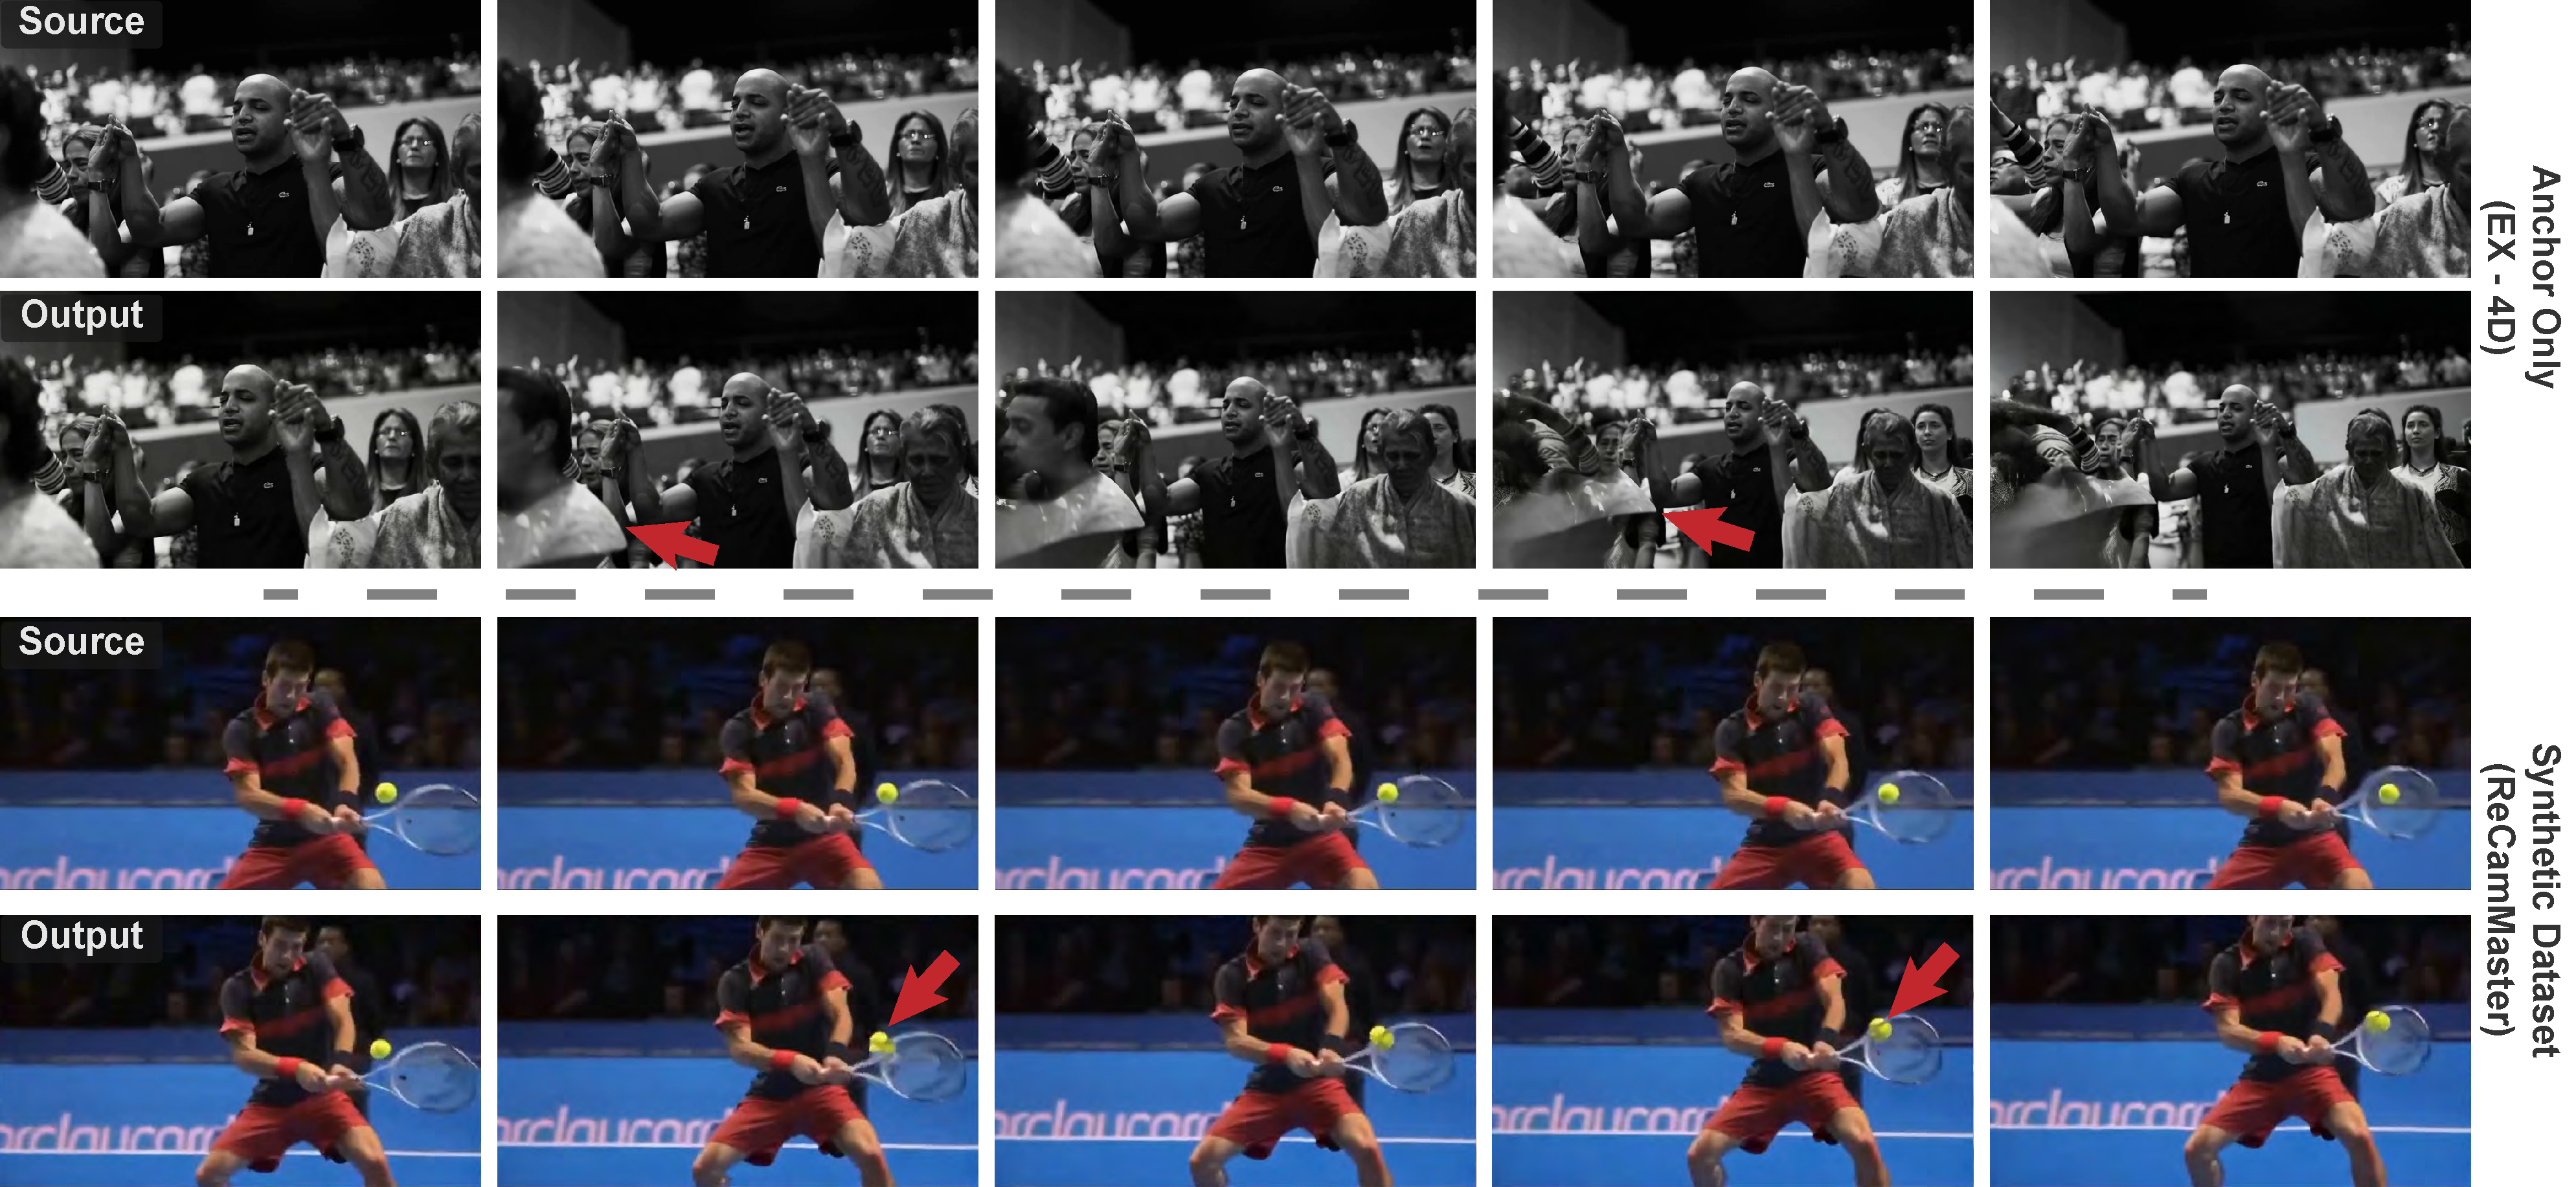
\includegraphics[width=\linewidth]{figures/supp_motivation.pdf}
    % \vspace{-0.25in}
\captionof{figure}{\textbf{Motivation: Illustrating Failure Modes in Video Reshooting.} This figure highlights common limitations of existing video reshooting methods, motivating our approach.
\textbf{(Rows 1-2) Anchor-Only Artifacts:} Given a high-quality source video (Row 1), an anchor-only method like \exfd{}~\cite{ex4d} (shown in Row 2) often generates significant ghosting and content inconsistencies. This occurs when the model relies solely on an imperfect anchor video ($V_a$) for geometric guidance and struggles to hallucinate complex details not fully represented in $V_a$.
\textbf{(Rows 3-4) Loss of Detail in Synthetic-Data Models:} For a given source video (Row 3), synthetic-data trained models, such as \recammaster{}~\cite{bai2025recammaster} (Row 4), can fail to capture intricate spatio-temporal details and object dynamics. In this example, \recammaster{} incorrectly deforms the tennis ball as it moves across the racket.
\textit{Note on \recammaster{}:} While \recammaster{} demonstrates impressive capabilities in general camera-controlled video generation, this result (obtained from the demo videos on their official project website) highlights that challenges with intricate object dynamics persist even in their best demonstrations, and similar artifacts are evident in their other results.}
    \label{fig:supp_motivation}
\end{center}
}
]


\begin{figure*}
    \centering
    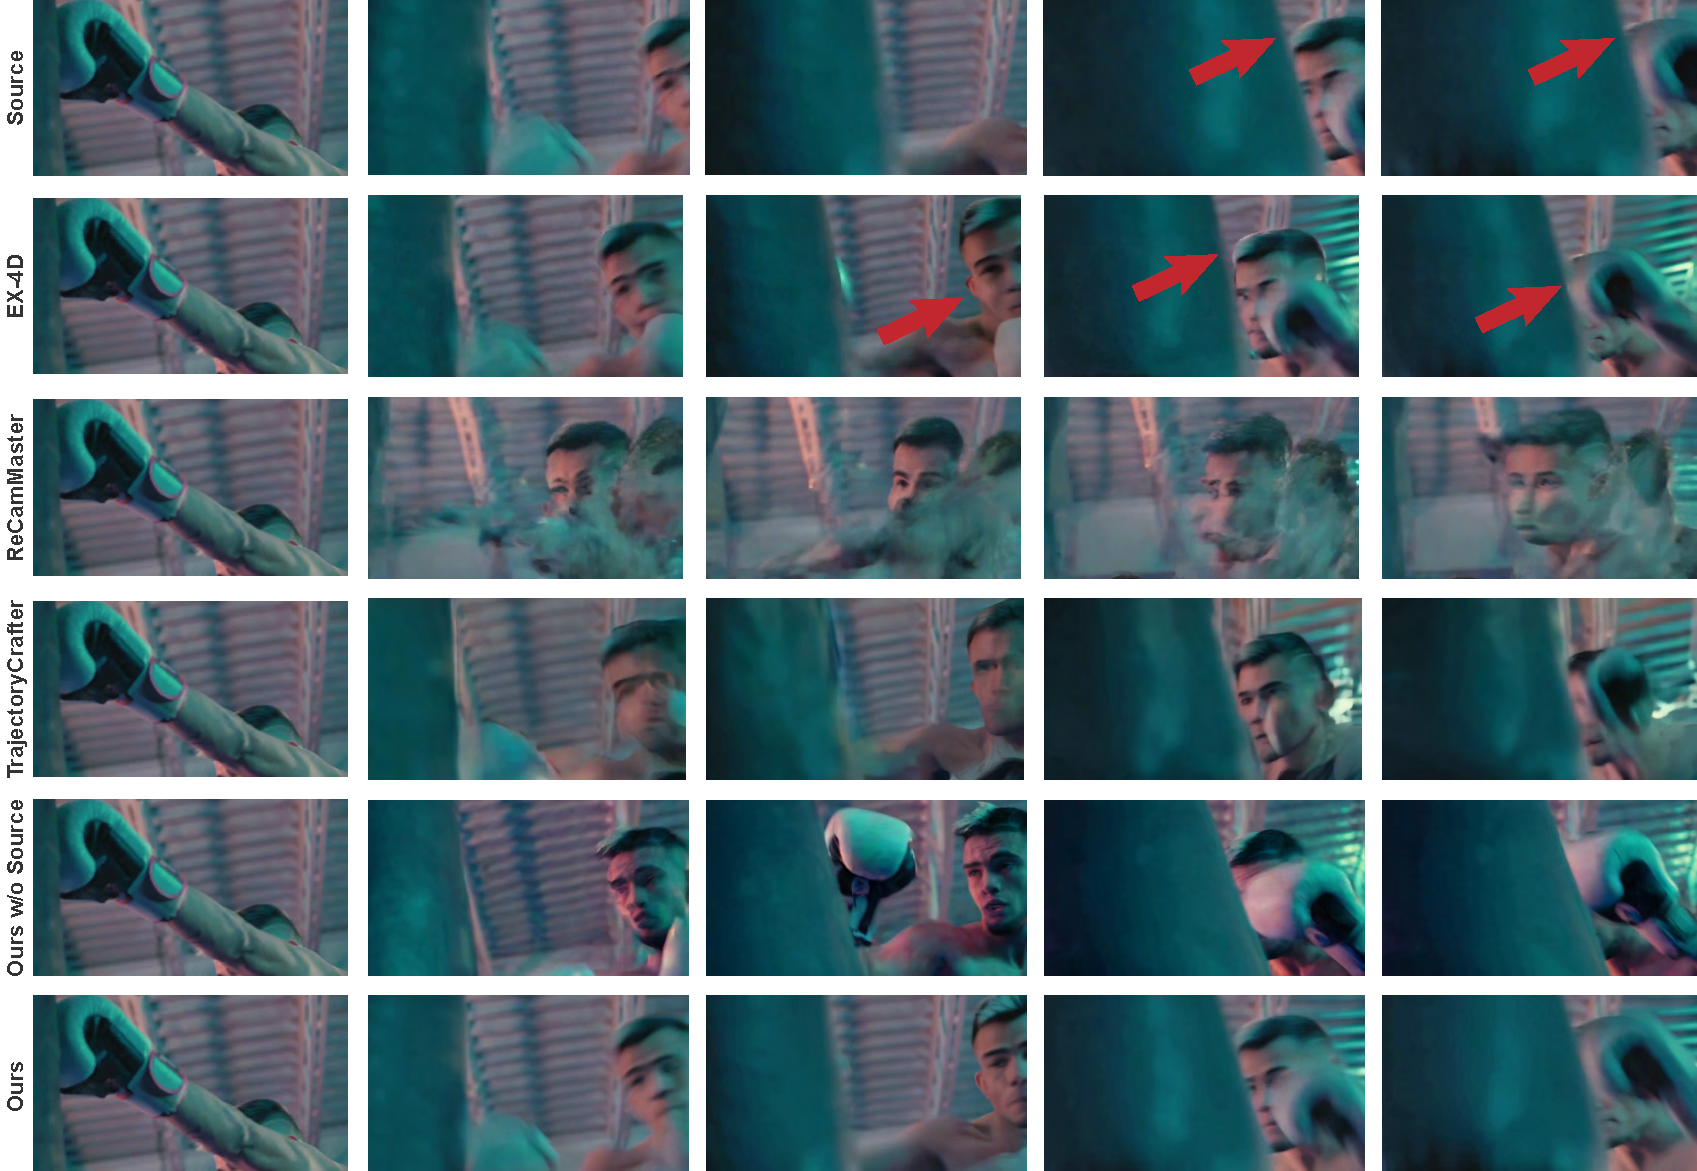
\includegraphics[width=\linewidth]{figures/supp_comp1.pdf}
    \vspace{-0.25in}
\caption{\textbf{Extended Qualitative Comparisons.} Each row displays sample frames from generated videos. Arrows indicate characteristic artifacts in baseline methods, such as loss of fine detail, blurring, or texture distortion. In contrast, our approach consistently demonstrates superior fidelity, accurately reproducing small details and effectively preserving intricate textures from the source video.}
    \label{fig:supp_comparison1}
    \vspace{-0.2in}
\end{figure*}




\begin{figure*}
    \centering
    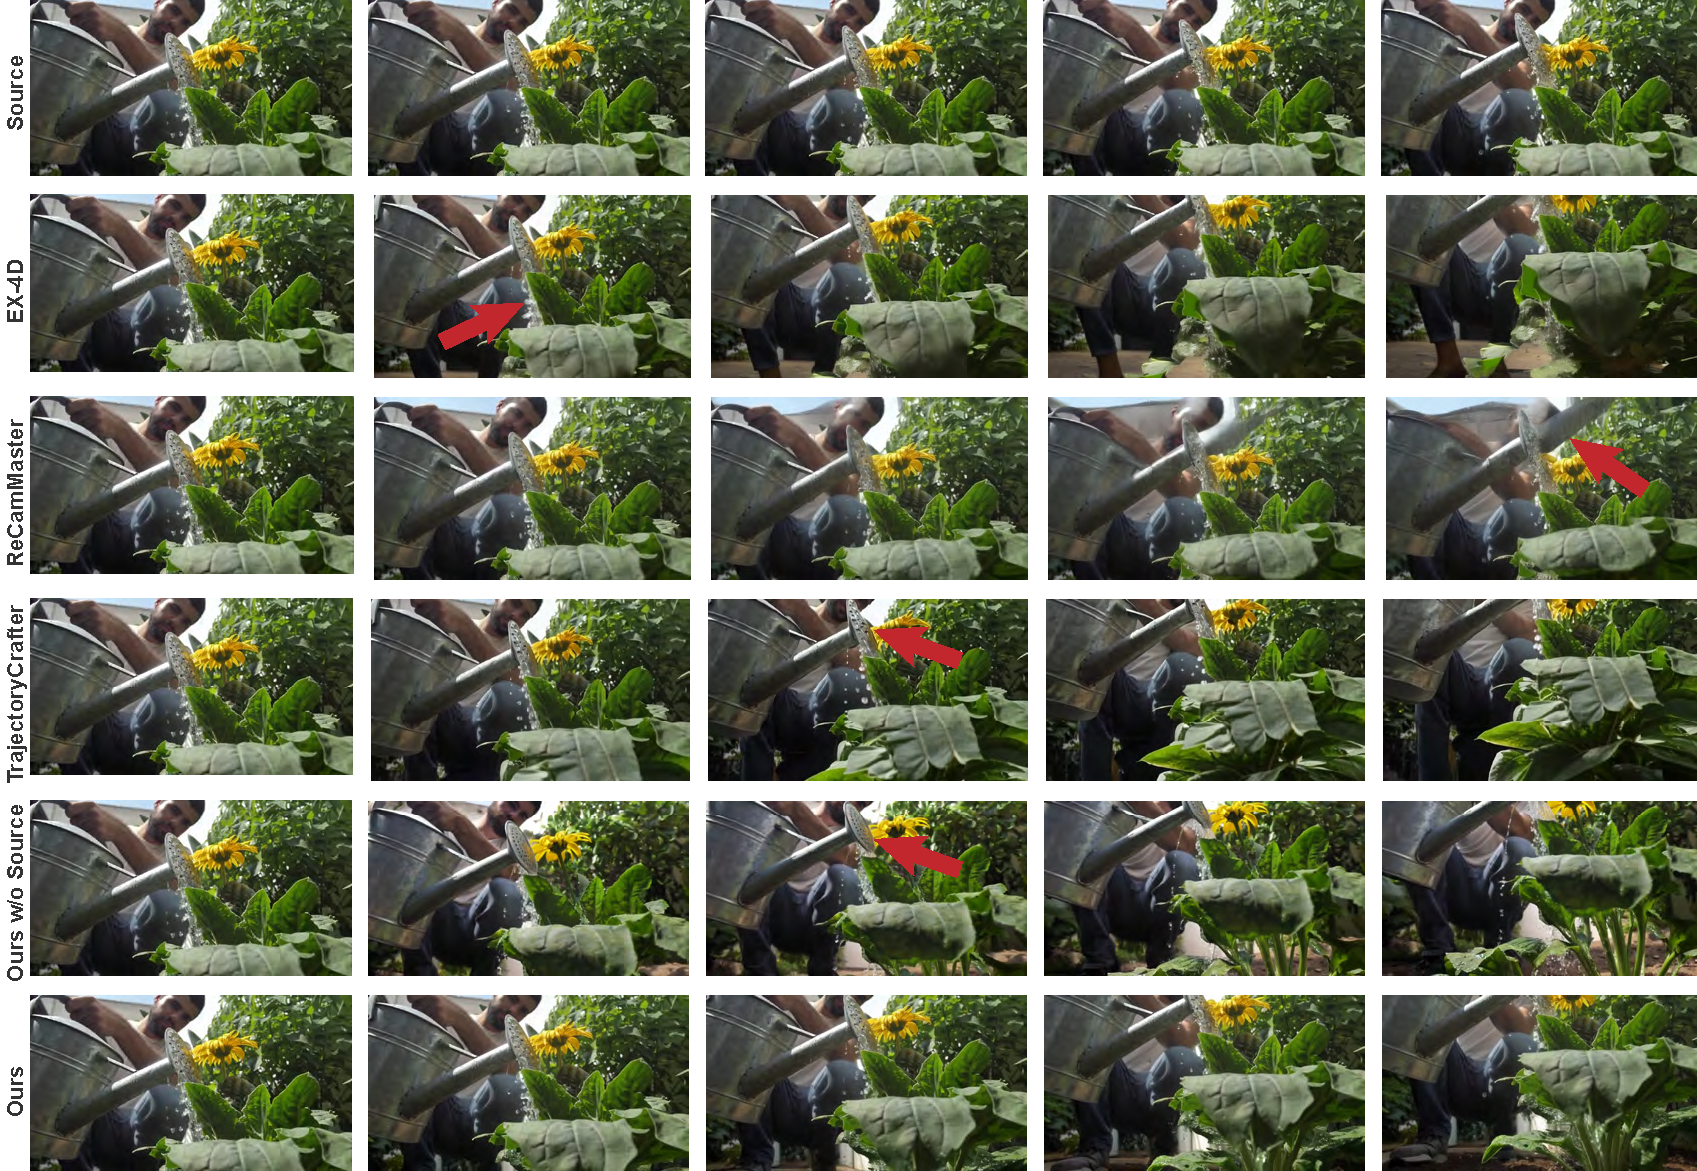
\includegraphics[width=\linewidth]{figures/supp_comp2.pdf}
    \vspace{-0.25in}
\caption{\textbf{Extended Qualitative Comparisons.} Each row displays sample frames from generated videos. Arrows indicate characteristic artifacts in baseline methods, such as loss of fine detail, blurring, or texture distortion. In contrast, our approach consistently demonstrates superior fidelity, accurately reproducing small details and effectively preserving intricate textures from the source video.}
    \label{fig:supp_comparison2}
    \vspace{-0.2in}
\end{figure*}



\begin{figure*}
    \centering
    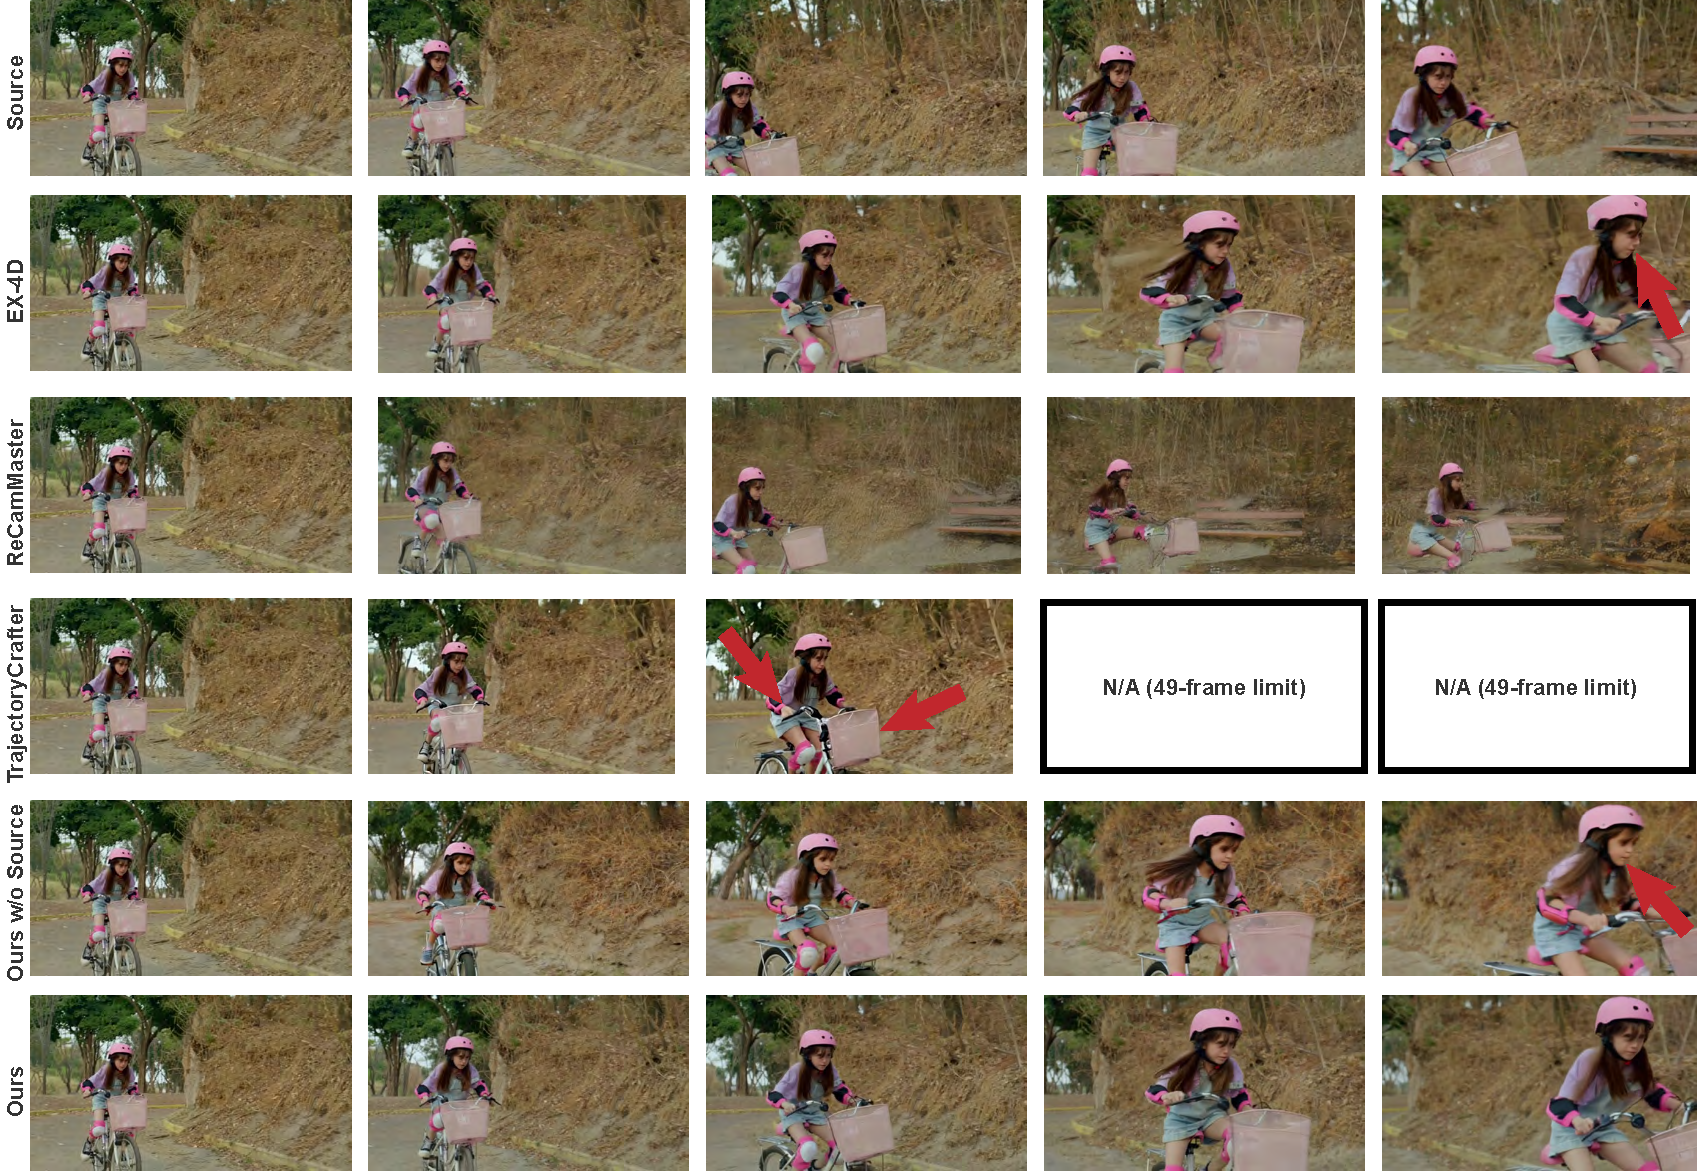
\includegraphics[width=\linewidth]{figures/supp_comp3.pdf}
    \vspace{-0.25in}
\caption{\textbf{Extended Qualitative Comparisons.} Each row displays sample frames from generated videos. Arrows indicate characteristic artifacts in baseline methods, such as loss of fine detail, blurring, or texture distortion. In contrast, our approach consistently demonstrates superior fidelity, accurately reproducing small details and effectively preserving intricate textures from the source video.}
    \label{fig:supp_comparison3}
    \vspace{-0.2in}
\end{figure*}



% \begin{figure*}
%     \centering
%     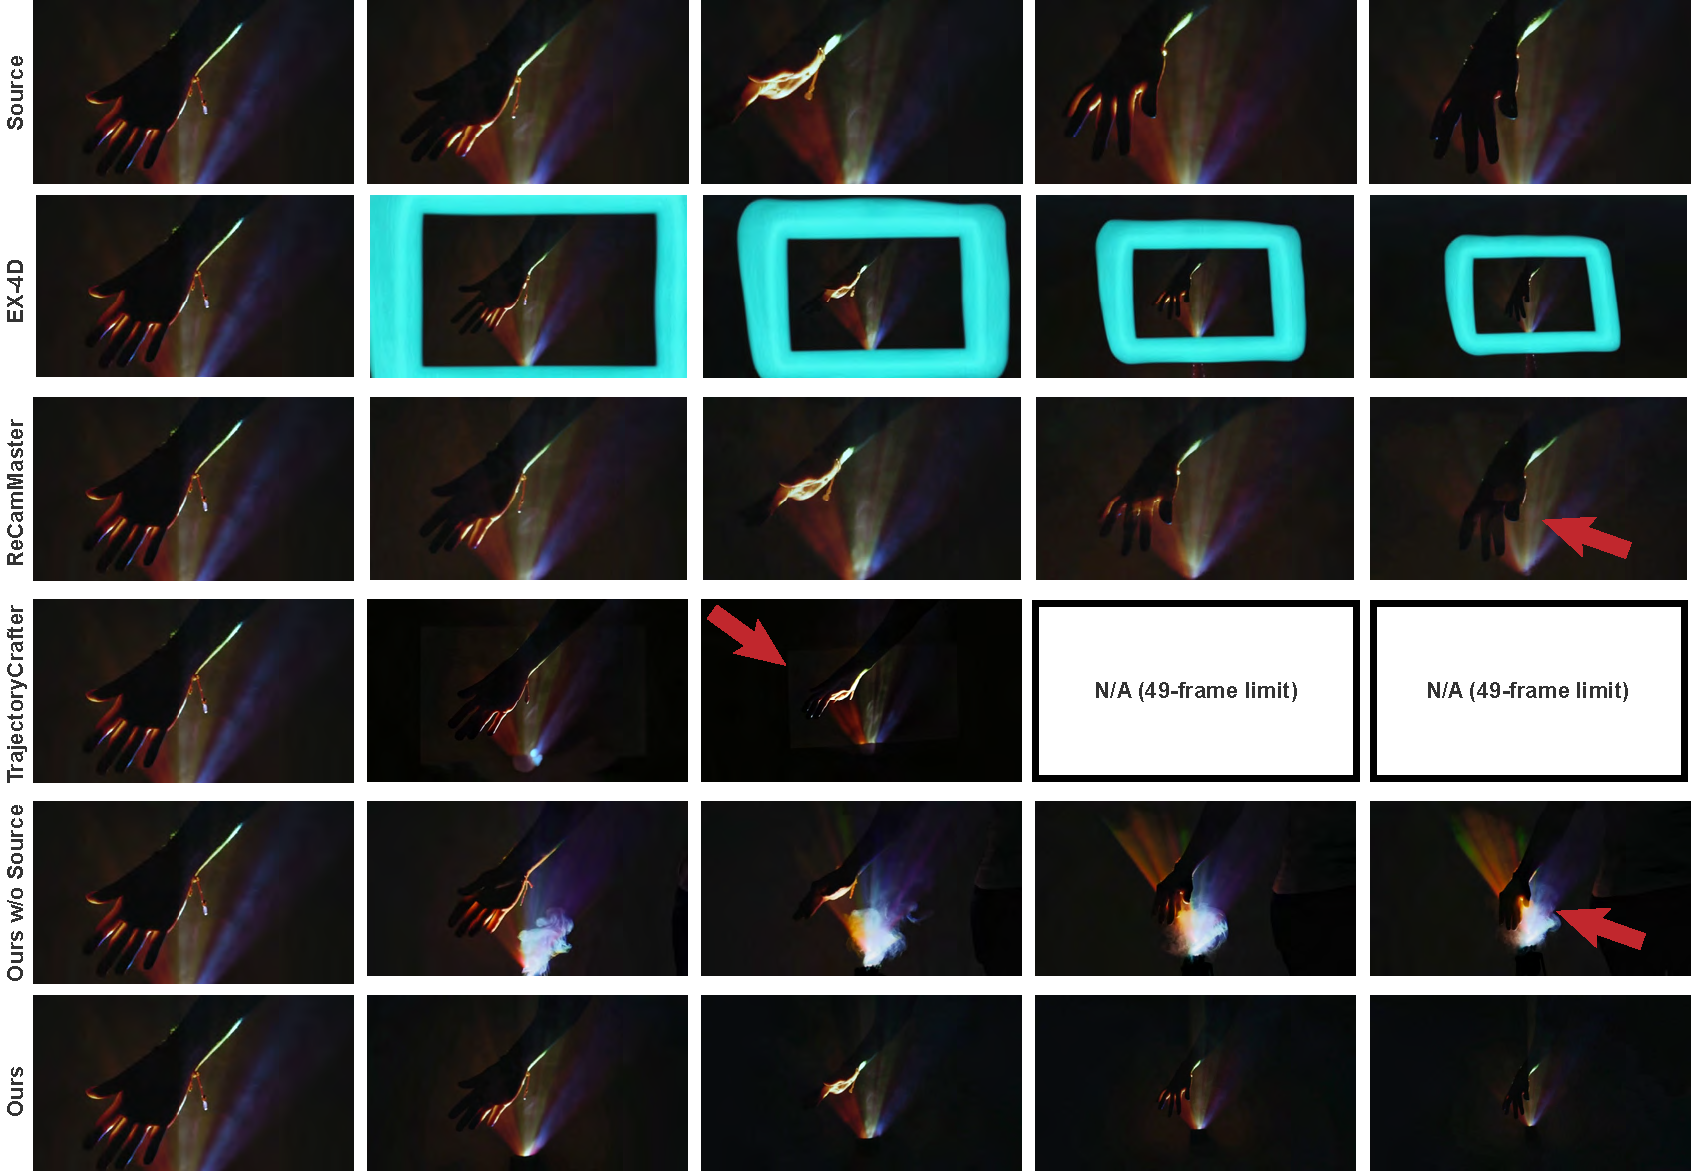
\includegraphics[width=\linewidth]{figures/supp_comp4.pdf}
%     \vspace{-0.25in}
% \caption{}
%     \label{fig:supp_comparison2}
%     \vspace{-0.2in}
% \end{figure*}



\begin{figure*}
    \centering
    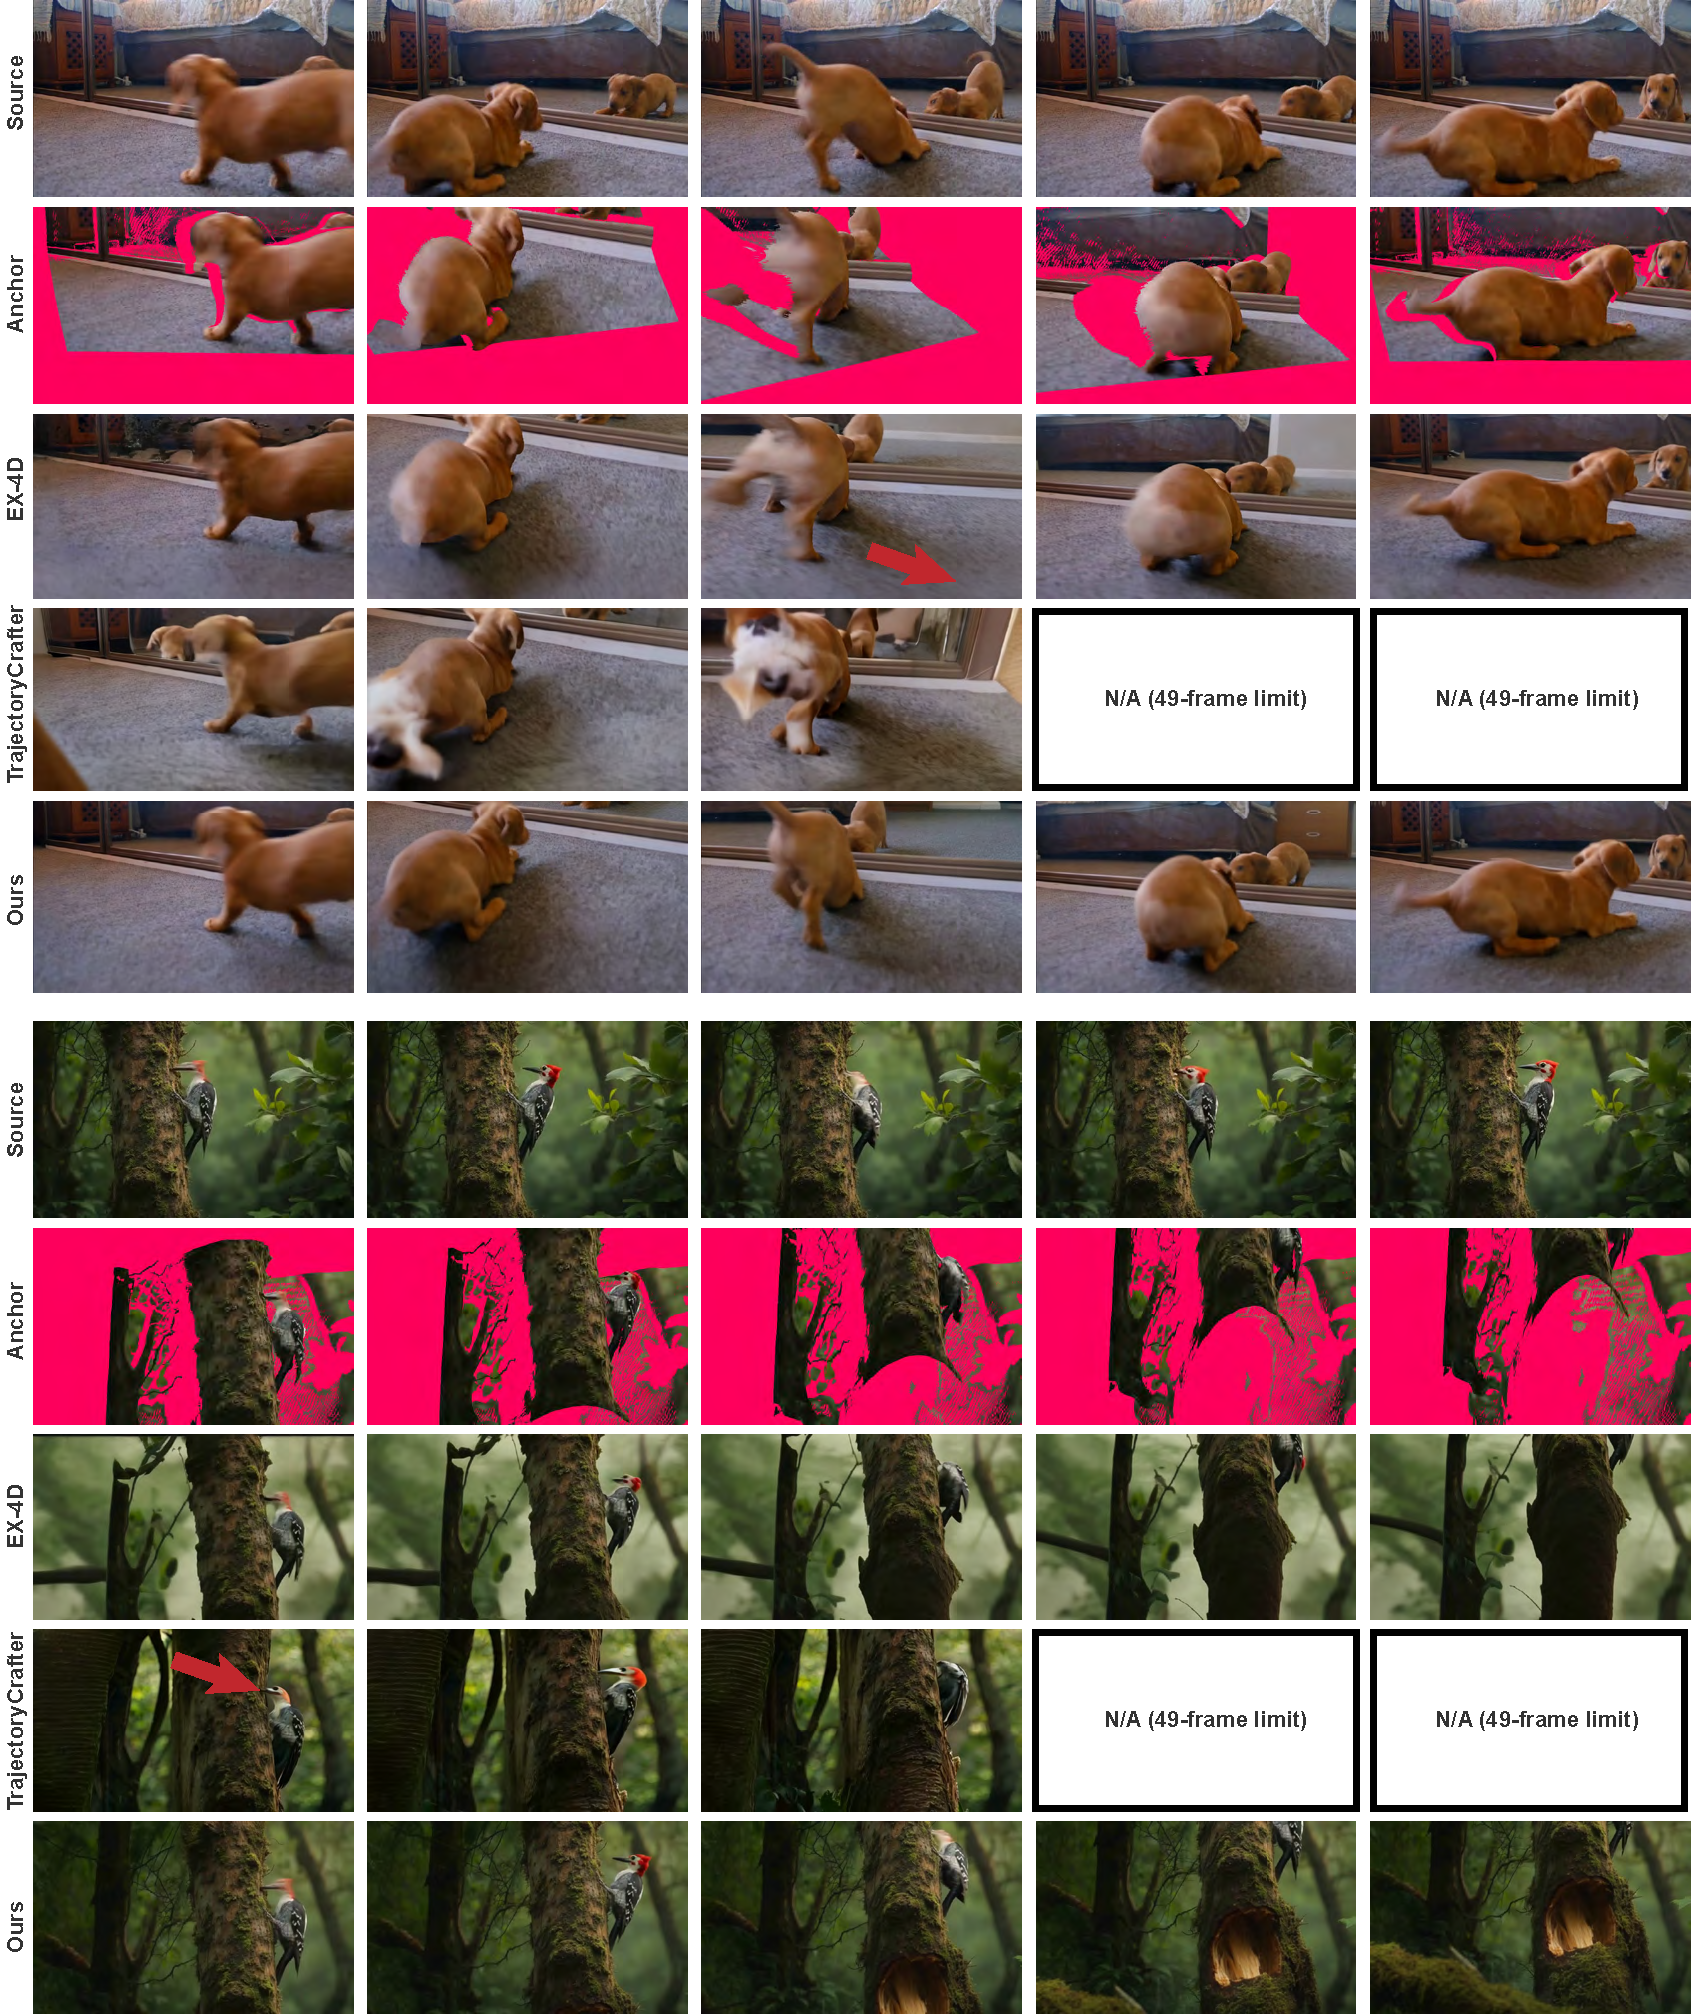
\includegraphics[width=\linewidth]{figures/supp_comp5.pdf}
    \vspace{-0.25in}
\caption{\textbf{Handling Random Camera Start Points while Maintaining Detail.} We illustrate anchor trajectories initiated from arbitrary viewpoints, causing significant spatial misalignment at the start of generation. Our model successfully handles these large initial viewpoint shifts without compromising quality, consistently preserving fine details and original textures in the generated video, even under such challenging conditions.}
    \label{fig:supp_comparison5}
    \vspace{-0.2in}
\end{figure*}




\begin{figure*}
    \centering
    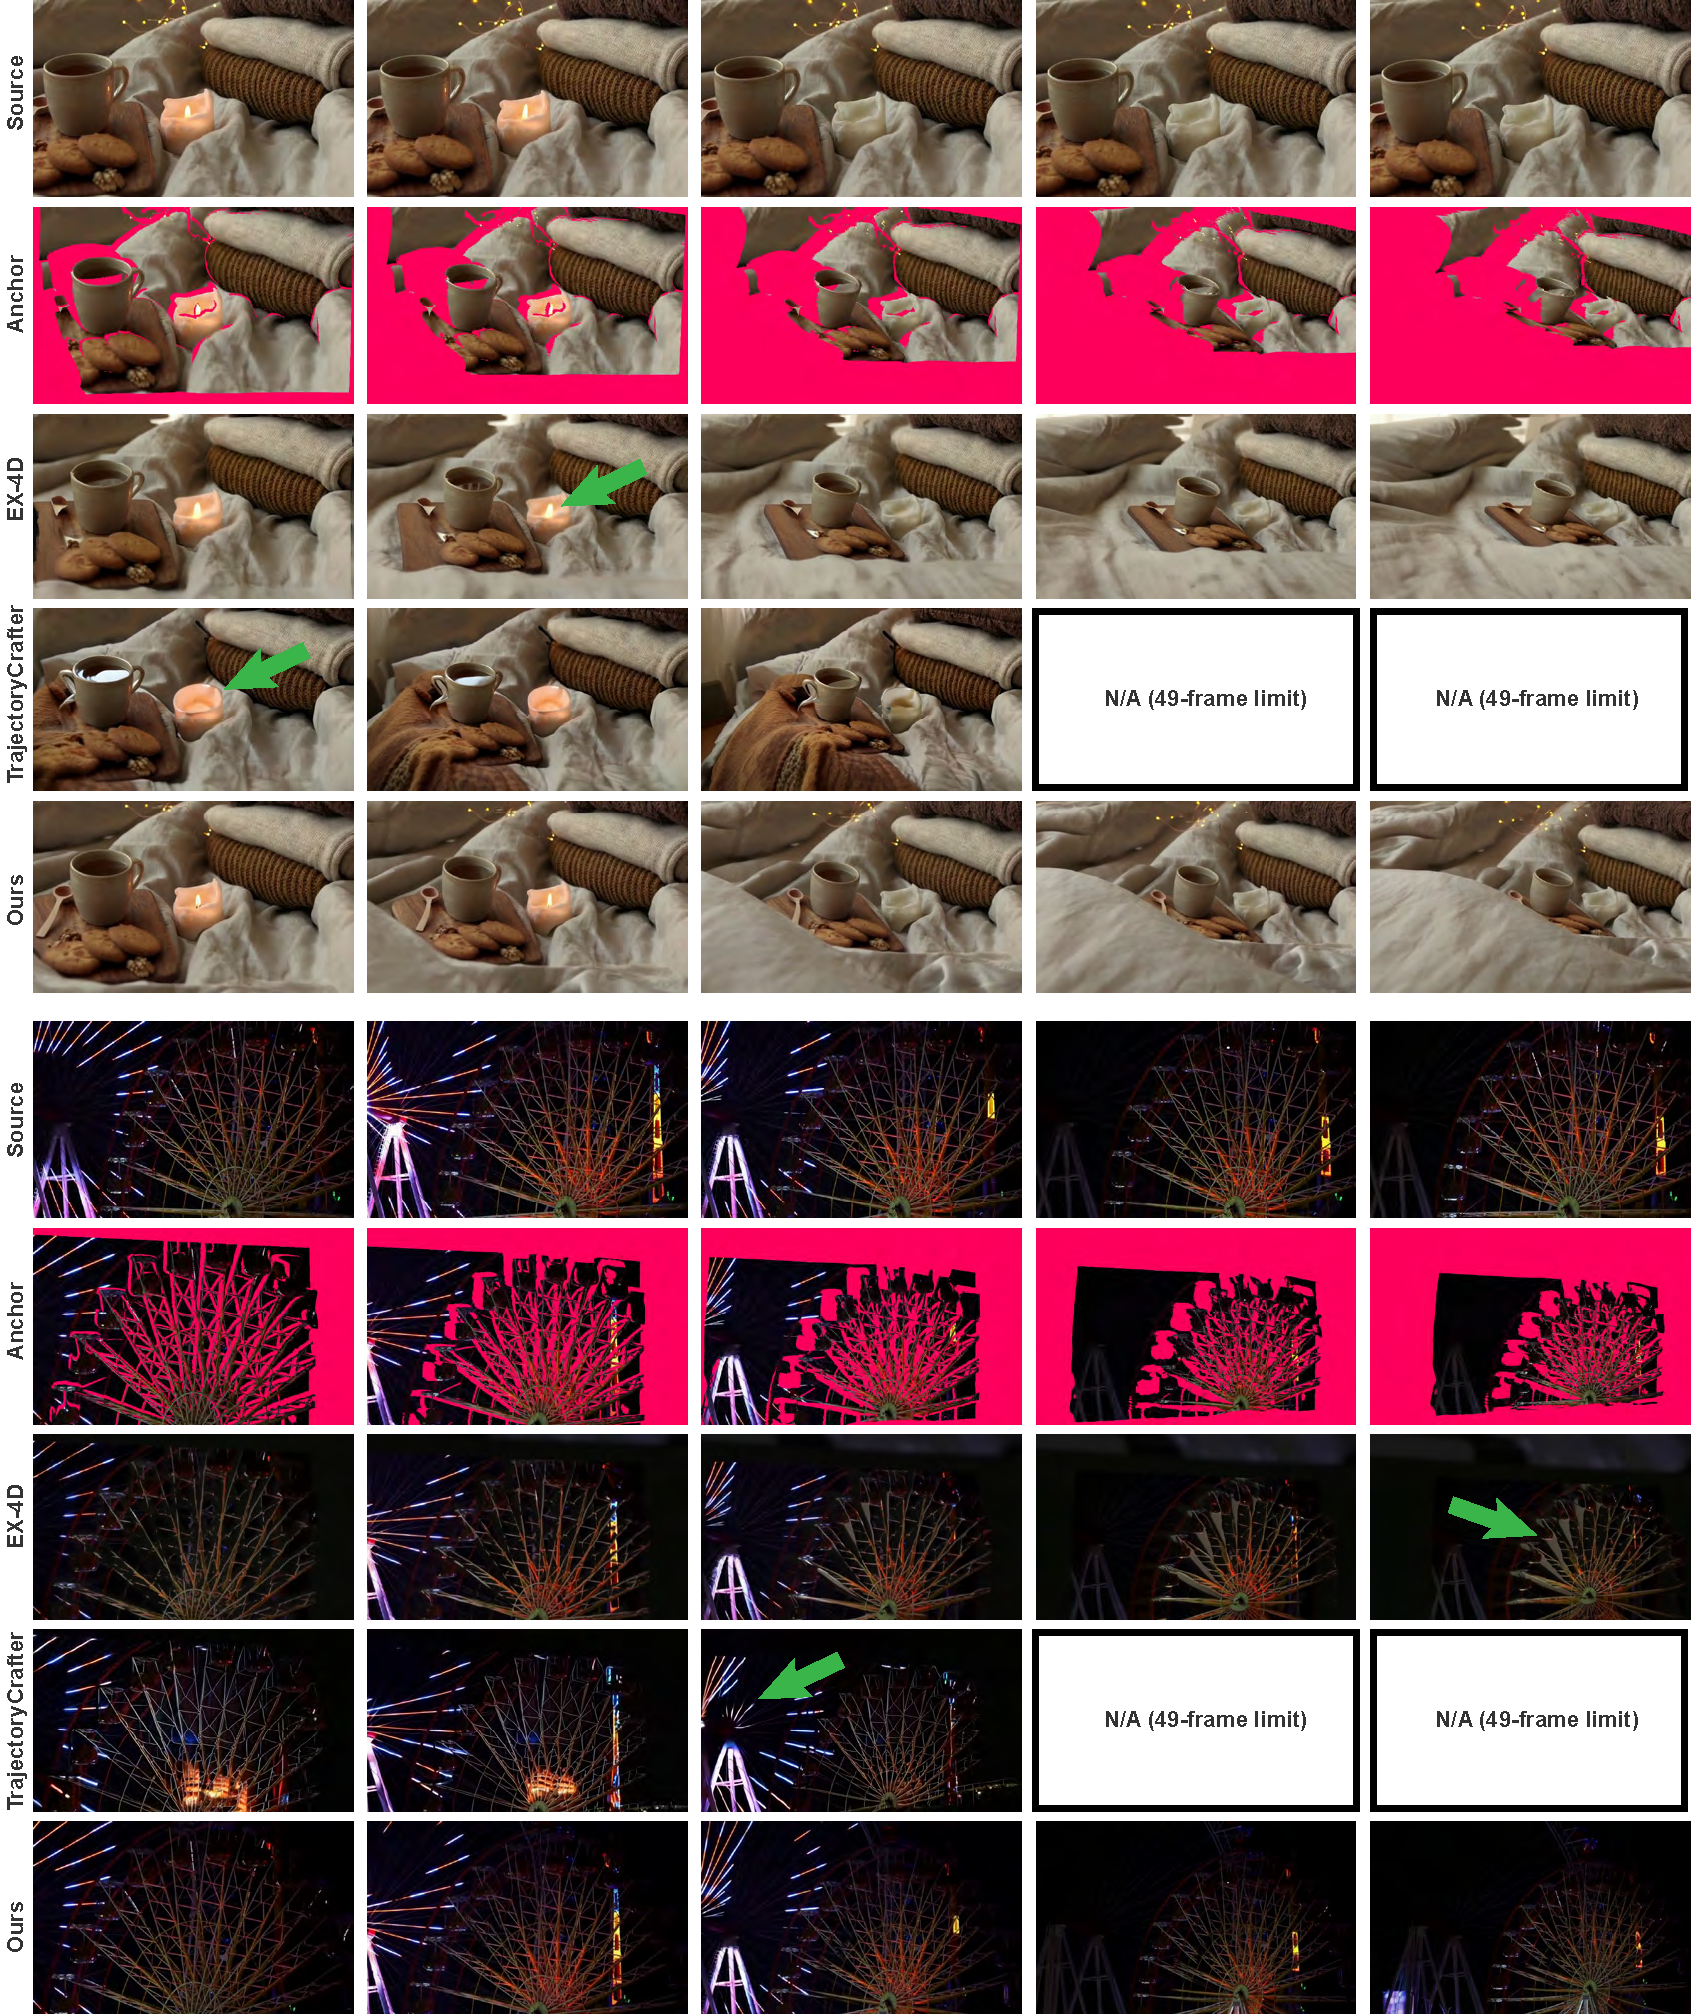
\includegraphics[width=\linewidth]{figures/supp_comp6.pdf}
    \vspace{-0.25in}
\caption{\textbf{Handling Random Camera Start Points while Maintaining Detail.} We illustrate anchor trajectories initiated from arbitrary viewpoints, causing significant spatial misalignment at the start of generation. Our model successfully handles these large initial viewpoint shifts without compromising quality, consistently preserving fine details and original textures in the generated video, even under such challenging conditions.}
    \label{fig:supp_comparison6}
    \vspace{-0.2in}
\end{figure*}




\begin{figure}
    \centering
    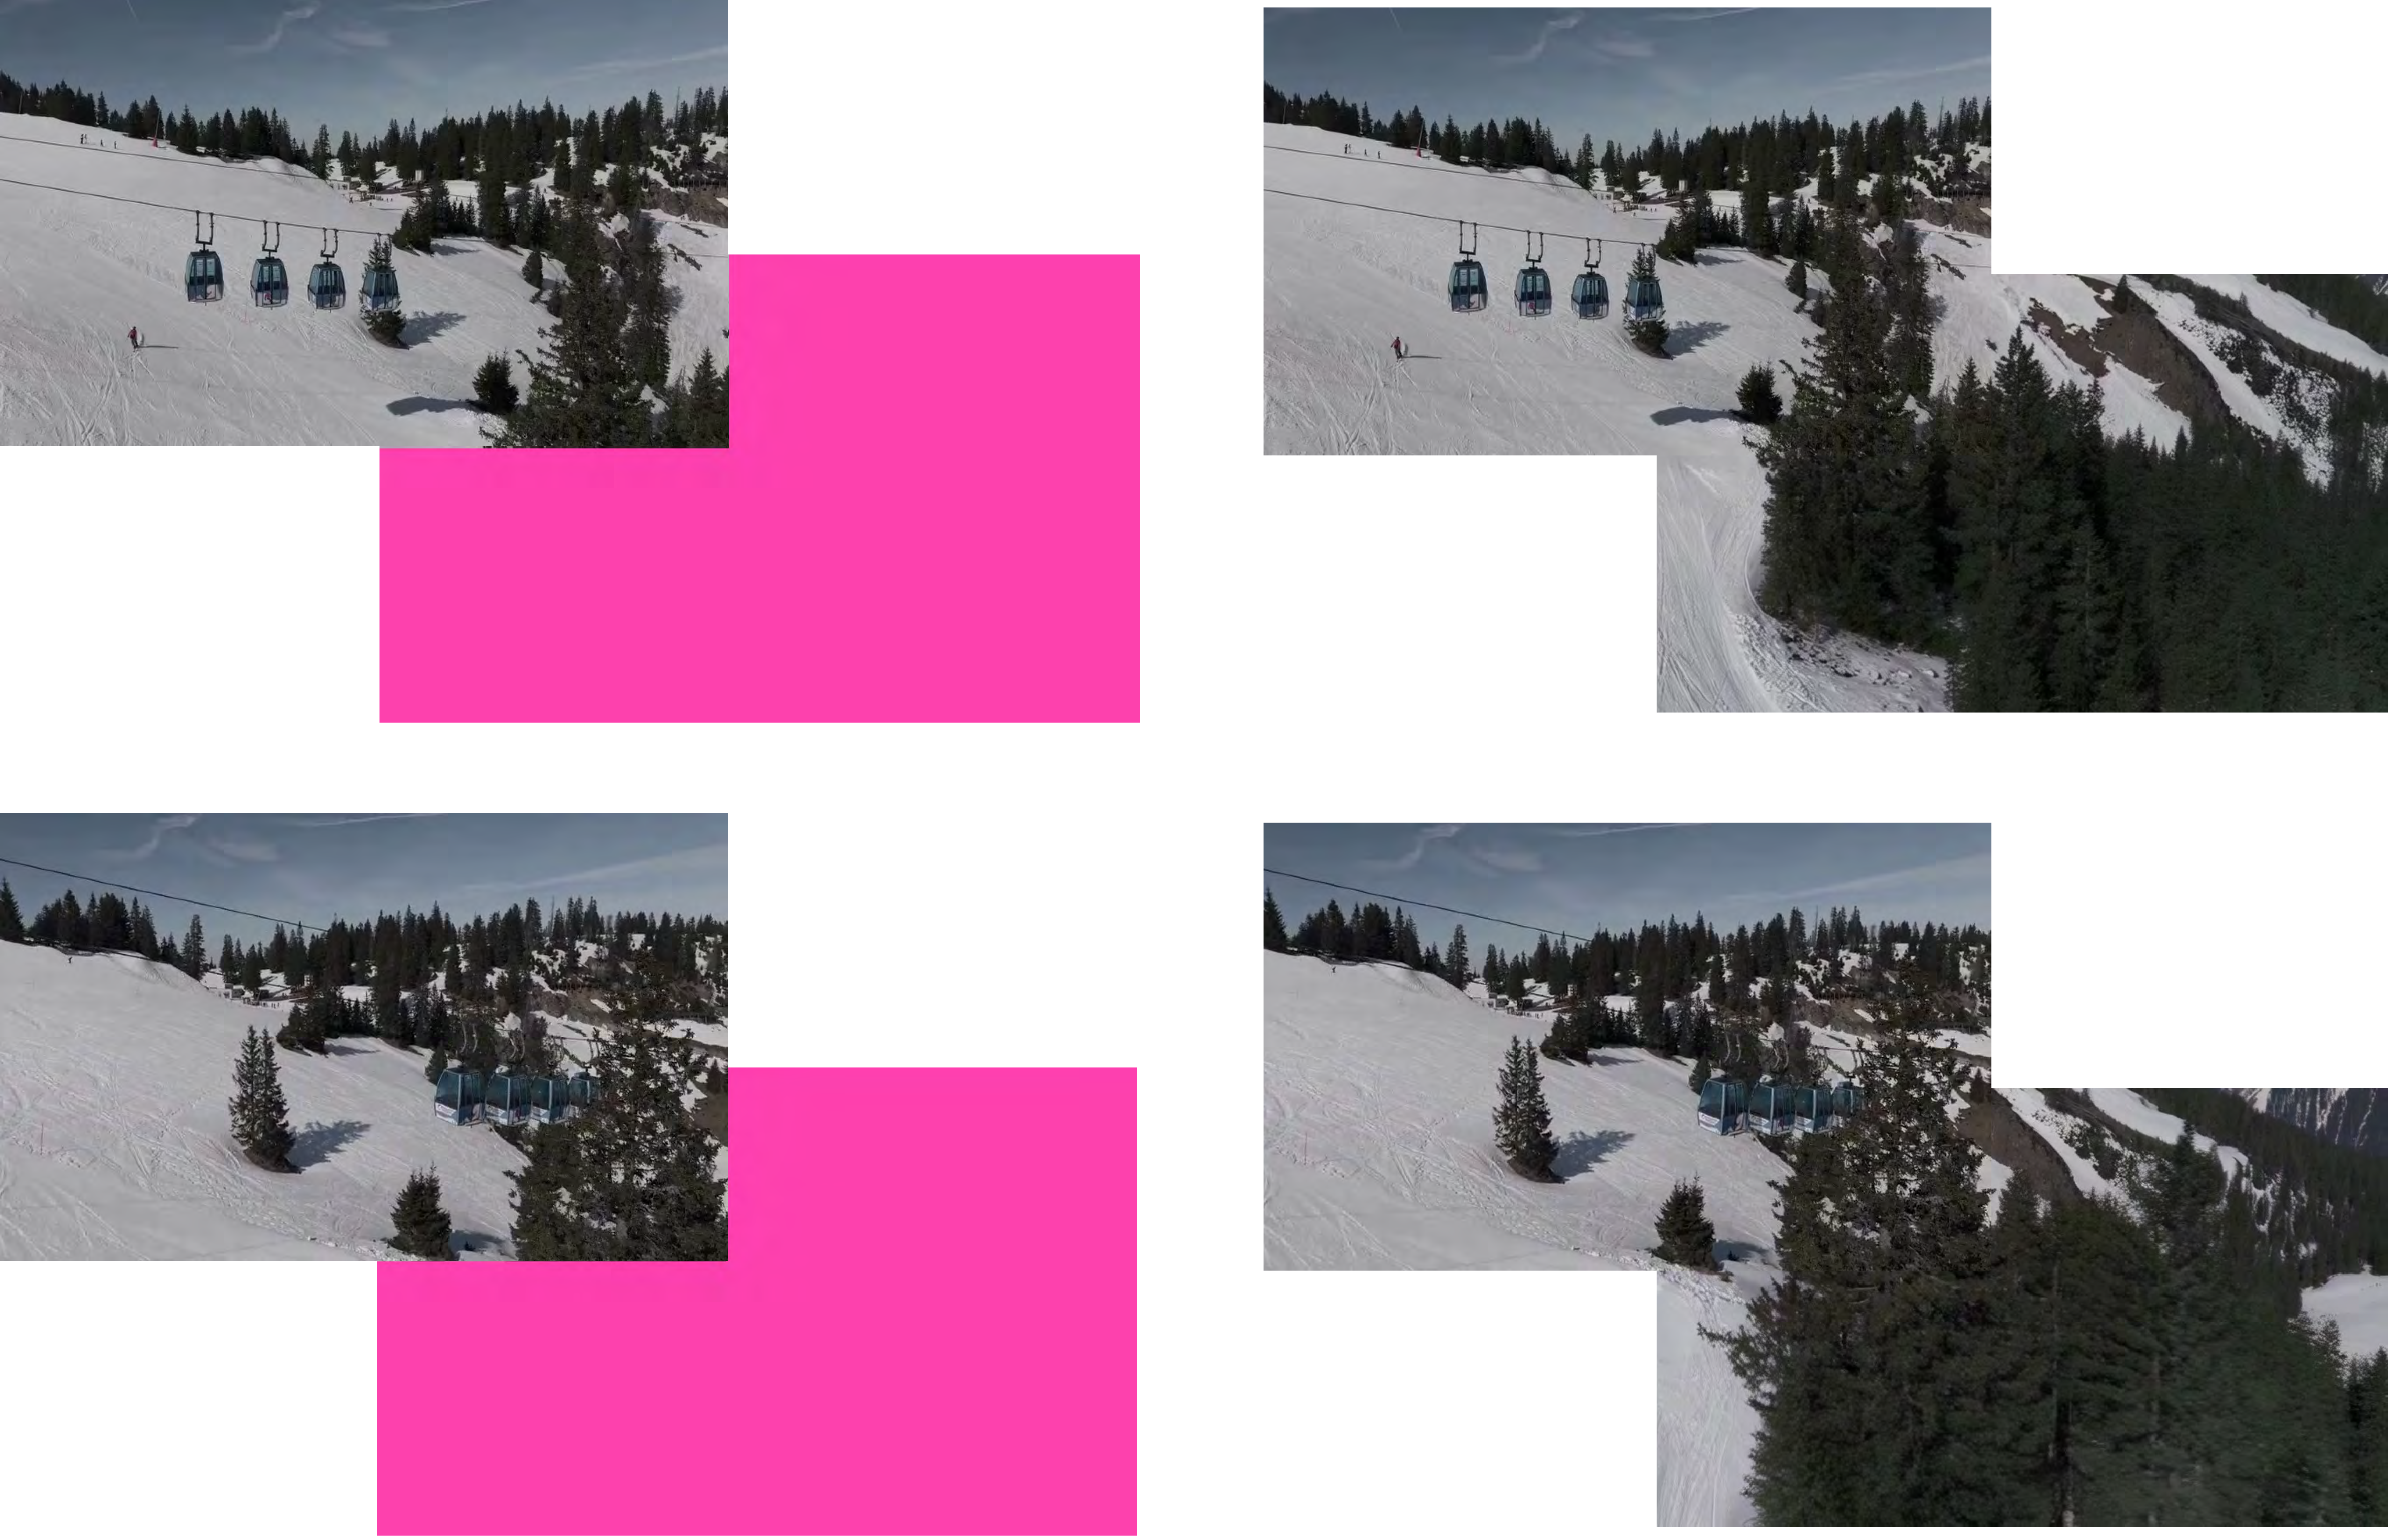
\includegraphics[width=\linewidth]{figures/supp_crop.pdf}
    \vspace{-0.25in}
\caption{\textbf{Extending Capabilities: Generative Outpainting.} Beyond standard video reshooting based on anchor trajectories, our model demonstrates strong generative priors useful for outpainting tasks. In this example, a 2D crop window is shifted significantly towards the bottom-right, revealing a large unseen region. The model leverages its learned priors to plausibly "hallucinate" the missing content and coherently complete the scene.}
    \label{fig:supp_crop}
    \vspace{-0.2in}
\end{figure}




% \begin{figure}
%     \centering
%     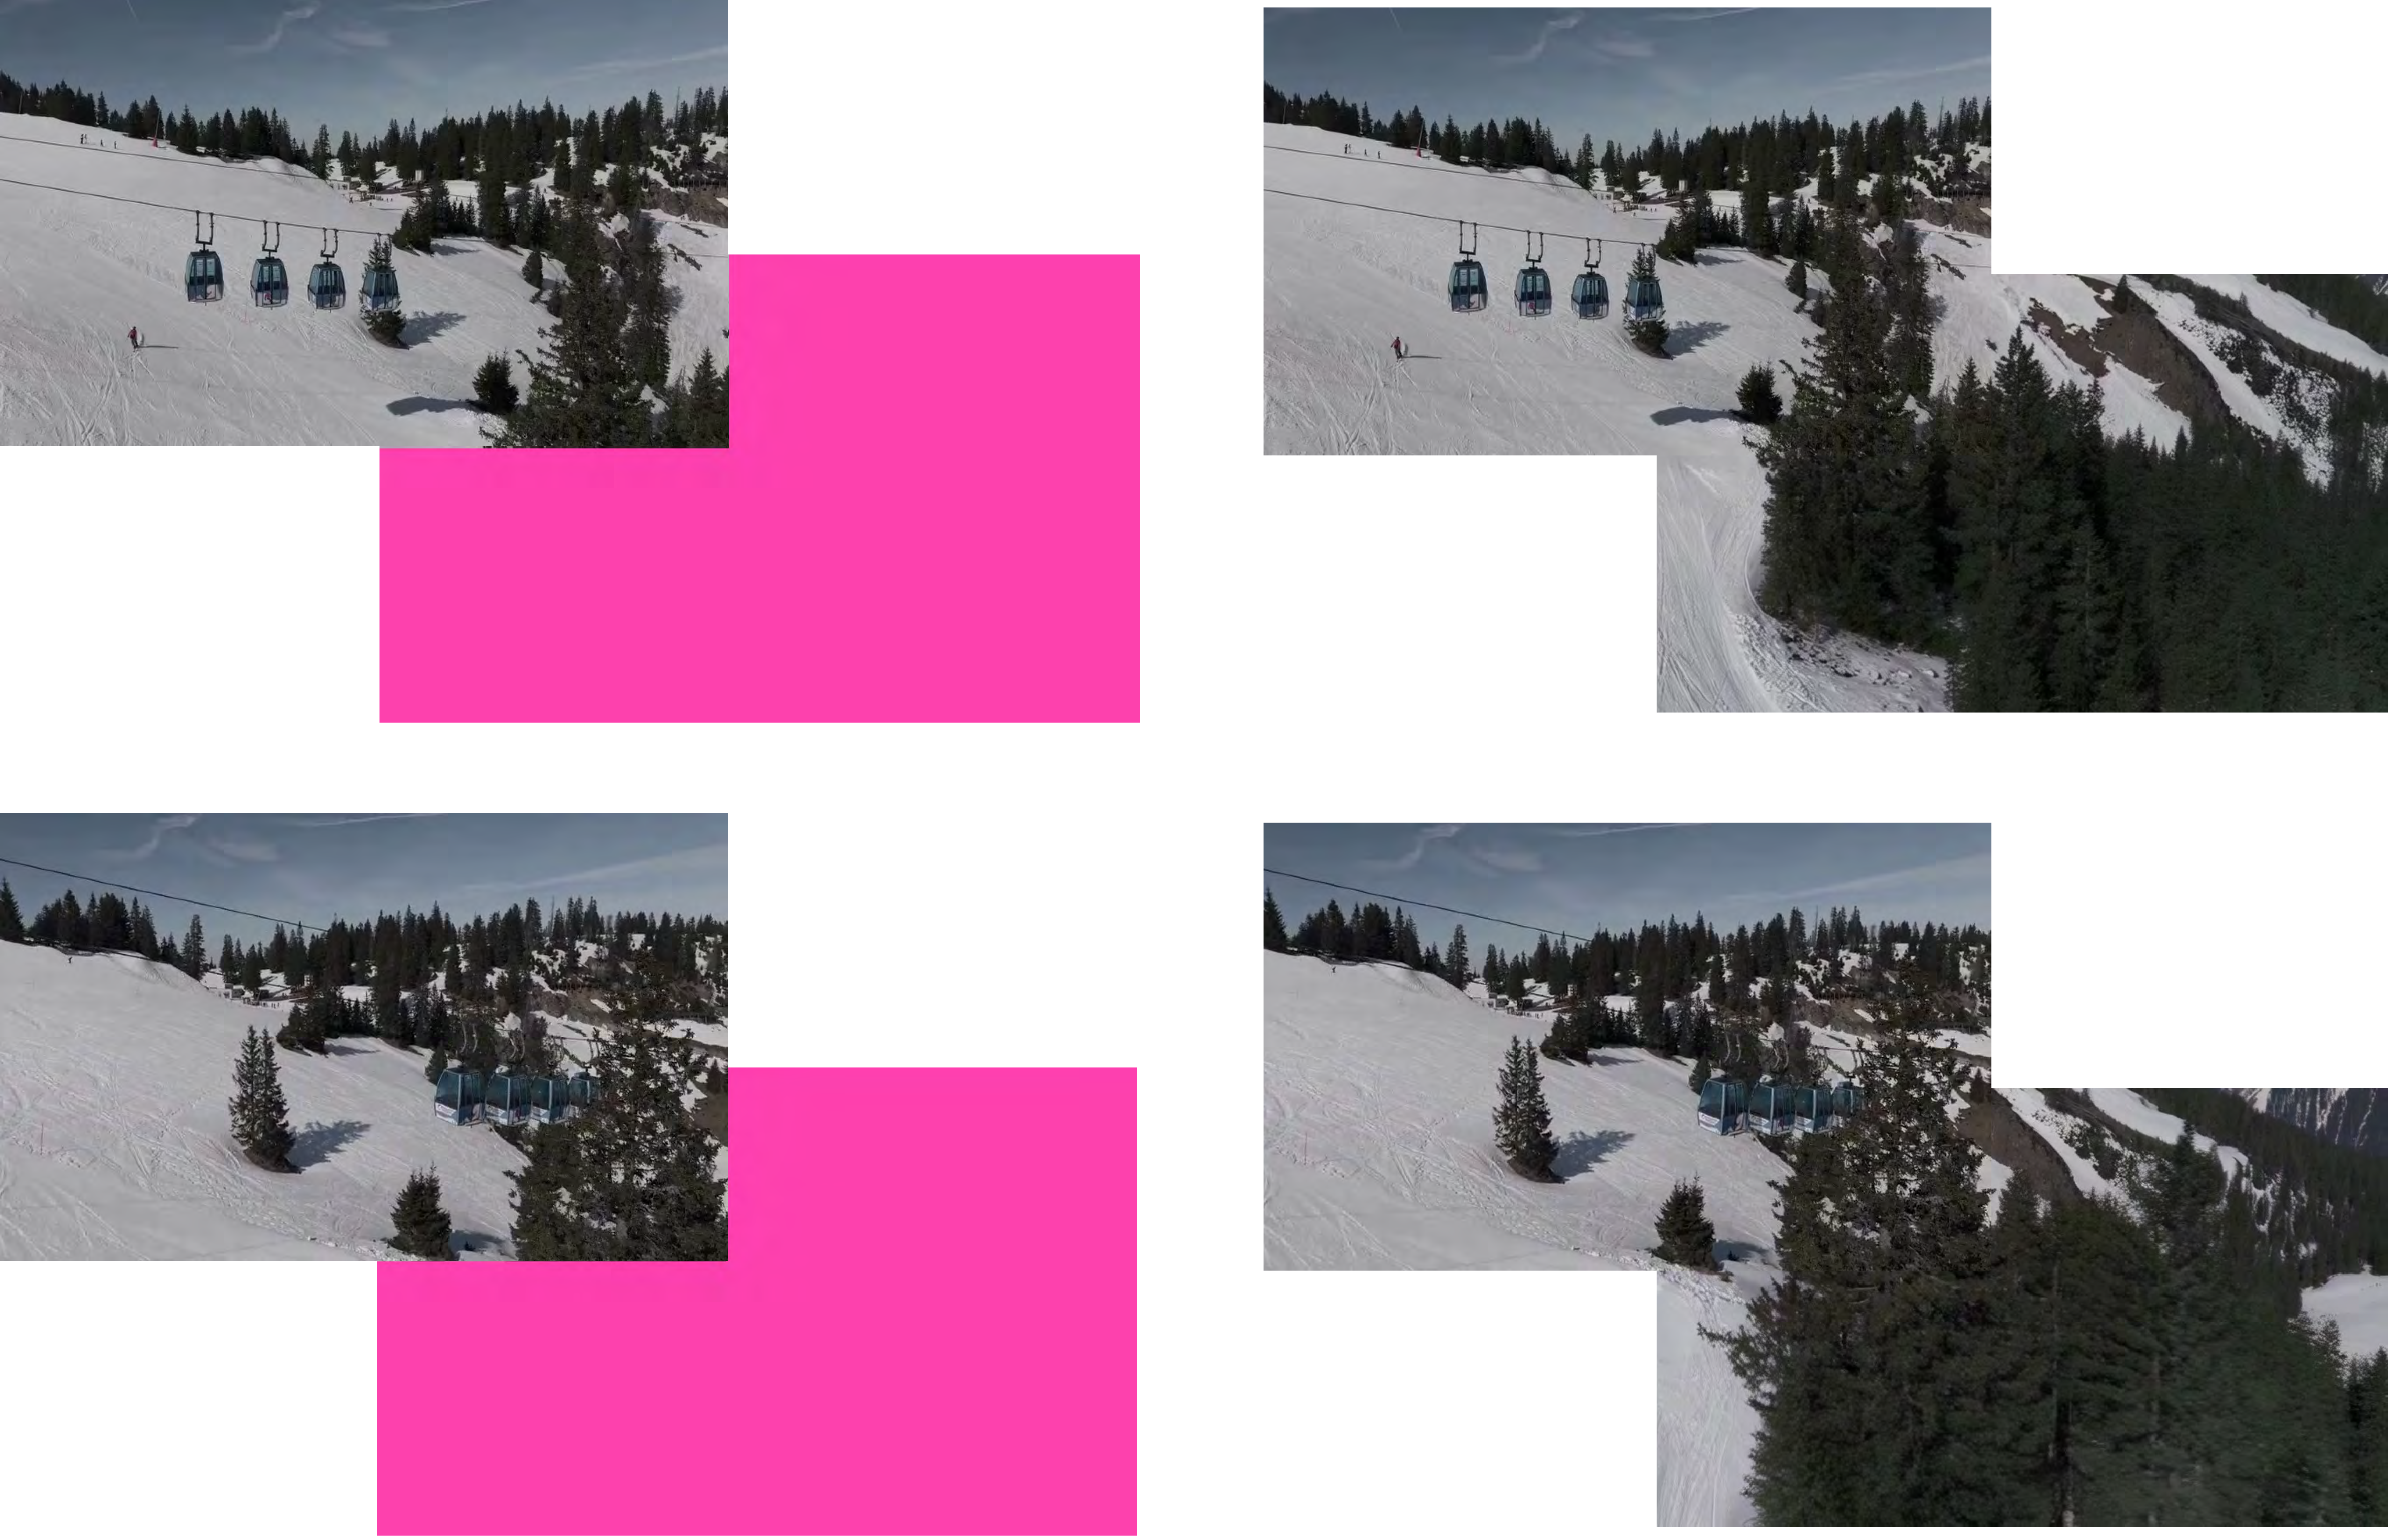
\includegraphics[width=\linewidth]{figures/supp_crop.pdf}
%     \vspace{-0.25in}
% \caption{\textbf{Extending Capabilities: Video Super-Resolution.} We demonstrate adapting our framework for video super-resolution. A low-resolution source video is simply upsampled to the target resolution (e.g., via bicubic interpolation) to serve as the anchor video ($V_a$). While this anchor lacks fine details, it provides coarse structural guidance. The model leverages its generative priors to synthesize plausible high-frequency textures consistent with the structure, producing a high-fidelity, high-resolution output.}
%     \label{fig:supp_crop}
%     \vspace{-0.2in}
% \end{figure}




In this supplementary material, we provide comprehensive implementation details, extended experimental results, and a discussion of potential applications for our video reshooting framework.


\section{Motivation} 
\label{sec:supp_motivation}

Achieving photorealistic video reshooting requires simultaneously maintaining precise geometric alignment with a novel camera trajectory while preserving the intricate textures and dynamic content of the original source video. Existing approaches often struggle to balance these requirements, leading to characteristic failure modes illustrated in Figure~\ref{fig:supp_motivation}. Methods that rely solely on sparse or imperfect anchor videos for conditioning, such as \exfd{}~\cite{ex4d}, are forced to "hallucinate" missing texture information without ground truth, frequently resulting in deformed texture or severe ghosting artifacts as seen in Rows 1 and 2. Conversely, models trained primarily on synthetic datasets, like \recammaster{}~\cite{bai2025recammaster}, often exhibit a domain gap when applied to real-world footage, failing to capture complex physical dynamics and fine-grained details, such as the rapidly moving tennis ball in Rows 3 and 4. These limitations collectively motivate our approach, which utilizes a self-supervised framework designed to learn directly from real-world monocular videos and explicitly fuses high-fidelity source texture with anchor-based geometric guidance to mitigate these issues.


\section{Implementation Details}
\subsection{Diffusion Transformer Configuration}
\label{sec:diffusion_transformer_config}

Our diffusion transformer is built upon the \textbf{Wan2.2-I2V 14B} model~\cite{wan21}. This specific base model employs a \textbf{Mixture-of-Experts (MoE)} design, featuring distinct parameter sets specialized for high-SNR (low-noise) and low-SNR (high-noise) regions of the diffusion trajectory. The architecture functions as a \textbf{Latent Diffusion Model (LDM)}, performing all video generation within a compressed latent space. Videos are encoded into a latent representation $z \in \mathbb{R}^{C_L \times T_L \times H_L \times W_L}$ by a causal 3D VAE with a U-Net backbone. This VAE temporally compresses the input, mapping the input video frames to $T_L$ latent frames.

The native Wan2.2 - I2V model is designed to condition on an image-reference latent (a VAE-compressed video where the first frame corresponds to the conditioning image and subsequent frames are typically zeroed), along with a binary mask indicating visible frame locations. Its standard conditioning pathway concatenates this image-reference latent, a $C_M$-channel binary mask, and a $C_L$-channel noisy latent along the channel dimension. This results in a tensor of shape $\mathbb{R}^{2C_L + C_M, T_L, H_L, W_L}$, which is then patchified and processed by the DiT transformer blocks. It utilizes \textbf{3D Rotary Positional Embeddings (3D-RoPE)} within its DiT blocks to encode spatiotemporal positional information.

For our video reshooting task, we adapt this conditioning scheme to integrate both anchor and source video information as described in the main paper.
\begin{description}[noitemsep, topsep=0pt, partopsep=0pt, leftmargin=1em, style=unboxed, font=\normalfont\bfseries]
    \item[Anchor Conditioning Stream] The VAE-encoded anchor latent $z_a \in \mathbb{R}^{C_L, T_L, H_L, W_L}$ is concatenated with a $C_L$-channel noise latent $z_n \in \mathbb{R}^{C_L, T_L, H_L, W_L}$ and a $C_M$-channel downsampled binary mask $M_a \in \mathbb{R}^{C_M, T_L, H_L, W_L}$. This forms a tensor with $2C_L + C_M$ channels, representing the anchor conditional input.
    \item[Source Conditioning Stream] The VAE-encoded source latent $z_s \in \mathbb{R}^{C_L, T_L, H_L, W_L}$ is duplicated along the channel dimension (effectively replacing $z_n$) and then concatenated with an all-ones $C_M$-channel mask $M_s \in \mathbb{R}^{C_M, T_L, H_L, W_L}$. This also results in a tensor with $2C_L + C_M$ channels.
\end{description}
These two conditional inputs (anchor and source streams) are then temporally concatenated, leading to a token sequence that is effectively twice as long as that used in standard I2V inference (i.e., $2 \times T_L$ latent frames). We share the parameters of the patchify blocks across both conditioning pathways.

To distinguish the positional context of the appended source tokens, we apply a constant offset to their \textbf{3D-RoPE} along the temporal dimension \textit{within the DiT blocks}. This offset magnitude is set to a fixed value of 50, which significantly exceeds our maximum number of training latent frames ($T_L=20$). This configuration allows us to flexibly change the length of generated videos during inference, as the source tokens are decoupled from the active denoising trajectory's temporal position. This large positional shift guides the model to interpret the source video tokens as temporally distinct, unlike methods such as~\cite{bai2025recammaster} where the RoPE offset typically matches the number of noisy latent frames and implies a continuous temporal sequence. The self-attention layers within the DiT blocks attend jointly over all concatenated anchor and source video tokens, enabling efficient cross-video knowledge transfer and improving temporal and structural consistency in generation.

For all experiments involving LoRA fine-tuning, we apply LoRA to all attention and fully connected layers. The conditioning setup remains consistent across both variants of the Mixture-of-Experts (MoE) DiT models.

\subsection{Augmentations and Ablation Setup}
\label{sec:augmentations_ablation_setup}

As introduced conceptually in the main paper, we implement several technical augmentations designed to further enhance model robustness, improve visual quality, and address specific challenges in video reshooting. These strategies are integral to achieving high-fidelity, consistent outputs. Here, we detail their specific configurations, the rationale behind them, and the contrasting setups used in our ablation studies (refer to Table 2 in the main paper).

\begin{description}[noitemsep, topsep=0pt, partopsep=0pt, leftmargin=0pt, style=unboxed, font=\normalfont\bfseries]
    \item[Source Token Reconstruction Loss] To ensure that the source token pathway actively retains meaningful content from the original source video, we apply an auxiliary reconstruction loss. During the backward pass, an L1 reconstruction loss is computed between the output tokens corresponding to the source video and the VAE-encoded clean source latent $z_s$. This loss is weighted by a factor of 0.1 and added to the primary diffusion loss. In ablations without this loss, this term is set to zero. This ablation is referred to as \textit{Auxiliary loss} in Table 2 of the main paper.

    \item[Anchor Background Treatment] In standard anchor video generation, regions representing new viewpoints or disocclusions are typically filled with a black background. However, for videos with dark scenes or objects, a black background can negatively interfere with generation, as the model may struggle to distinguish masked regions from actual dark content. To mitigate this, we evaluated different strategies:
    \begin{itemize}[noitemsep, topsep=0pt]
        \item \textit{Fixed Fluorescent:} Filling regions with high-contrast fluorescent pink. This provides a clear, distinct signal for the model, making the boundary of missing information unambiguous and potentially improving generation quality in challenging scenes.
        \item \textit{Random Color:} Filling regions with a single solid color sampled uniformly from the RGB cube per video.
    \end{itemize}
    Our empirical findings suggest that replacing the standard black background with a fluorescent, green-screen–like backdrop substantially reduces artifacts in dark scenes.

    \item[Flexible Anchor Reference Frame Warping] Our default anchor generation warps the first frame of the source video ($V_s[0]$) to create $V_a$. However, dense tracking methods allow for warping from any arbitrary reference frame. We introduce an augmentation where the reference frame for dense tracking and warping is randomly selected within the source video (e.g., $V_s[t]$ instead of always $V_s[0]$). This variability makes the training process more robust to diverse tracking conditions and improves the model's ability to handle anchor videos generated from various reference points (instead of having to match the first frame of the source video). Furthermore, this prevents the model from developing a bias towards early frames, which often exhibit higher quality in long-range warping. By forcing the model to attend to anchors derived from various points in time, it encourages sustained attention to the anchor's geometric guidance throughout the entire video. In our ablation study, this is referred to as \textit{Random Query} in Table 2 of the main paper, and we compare it against a baseline where the reference frame is fixed to the first frame ($V_s[0]$).

    \item[3D-Aware Noise Injection vs. Latent Noise] A potential issue arises when the synthesized anchor video ($V_a$) closely resembles the target video ($V_t$), tempting the model to "cheat" by directly copying texture from $V_a$ instead of sourcing from $V_s$. This can lead to overfitting on $V_a$'s texture, making the model overly reliant on its potentially inaccurate content during inference. To suppress $V_a$'s texture information while preserving its crucial 3D geometric guidance, our final strategy injects Gaussian noise into the RGB values of the reference frame ($V_s[t]$) \textit{before} it is forward-warped to create $V_a$. The noise magnitude is sampled from a uniform distribution between [0, 0.5] (on normalized [0, 1] RGB images) per channel. This creates a noisy anchor where the noise pattern appears to be \textit{stuck} to the surface. Unlike injecting noise \textit{after} warping (which would obscure motion cues by making per-frame textures independently noisy), pre-warping noise ensures that the noise itself moves coherently with the underlying 3D structure. This allows the model to still infer motion and geometry from the noisy $V_a$, but prevents it from directly copying texture, thereby forcing it to rely on $V_s$ for high-fidelity content. We contrast this with the common approach of adding independent standard Gaussian noise directly to the encoded anchor latents ($z_a$) \textit{after} VAE encoding. Injecting 3D noise into the anchor trajectory during training further improves robustness to imperfections in the underlying 4D reconstructions.
\end{description}

\noindent \textbf{Structural Ablations:} In addition to these augmentations, we also evaluated structural choices. We compared \textbf{LoRA Fine-tuning} (rank-512 on attention/FFN layers plus patchify) against \textbf{Full Fine-tuning}. Empirically, we find that incorporating LoRA during training improves generalization and stability, and we therefore retain this strategy for our final model. We also evaluated the necessity of the source stream by training a \textbf{No Reference Video} baseline, where the source conditioning stream is omitted.


\subsection{Anchor Generation for Inference}
\label{sec:inference_anchor_gen}

While our self-supervised training pipeline utilizes efficient 2D warping for anchor generation, during inference we utilize an explicit 3D projection approach to define the target camera trajectory. To generate an anchor video frame $V_a[t]$ at inference time, we first extract dense geometric information from the source video sequence, utilizing state-of-the-art monocular video depth and camera estimation models to obtain per-pixel depth maps and the camera trajectory for every frame~\cite{huang2025vipe, xu2025geometrycrafter, 4d_recon_hu2025depthcrafter}. Next, using these estimated depth maps and camera parameters, we unproject the source video frame pixels into world 3D space, resulting in a consistent and dense, colored point cloud representation of the underlying scene geometry. Finally, to generate an anchor frame corresponding to a specific target camera pose, we re-render this 3D point cloud from the novel viewpoint. We utilize the input cameras to cancel out the original video's camera motion.


\subsection{Evaluation}

\textbf{Dataset}
To establish a representative evaluation benchmark, we constructed a final set of 100 videos, sub-sampled from the initial pool of 1,000 stratified examples from the Opensora-mixkit dataset~\cite{lin2024open}. This curation process was designed to balance semantic coverage, camera motion diversity, and occlusion characteristics. First, videos were randomly assigned 1 of 10 predefined camera motion trajectories provided by \recammaster{}~\cite{bai2025recammaster}. After generating the anchor videos, we quantified the extent of motion and disocclusion by calculating the mean value of the generated anchor mask ($M_a$) for each video. To ensure balanced movement representation, videos were grouped by trajectory, and the median mask value was determined for each group. Finally, we selected the 10 videos nearest to their respective group median. This sampling strategy mitigates outliers with extreme mask presence (too static or empty anchors due to depth estimation errors), preserving the underlying semantic distribution while ensuring a representative mix of movement characteristics across all camera trajectories.



\noindent\textbf{Metrics}
For video-to-video models, we follow \recammaster{}~\cite{bai2025recammaster} and evaluate along three key dimensions: camera accuracy, view synchronization, and overall video quality. We present results from the VBench \cite{eval_huang2024vbench} benchmark for overall video quality, with an emphasis on per-video metrics such as Subject Consistency, Motion Smoothness, Aesthetic Quality, Temporal Flickering, Imaging Quality, and Background Consistency. Furthermore, to evaluate the temporal consistency of the frames of the generated videos, we compute CLIP-F as in \cite{bai2025recammaster}, which is the average CLIP similarity score of
the adjacent frames. 


We used metrics from ~\cite{camera_traj_he2024cameractrl} to measure both Rotational Error (RotErr) and Translational Error (TransErr) for camera accuracy. Using the ~\cite{huang2025vipe} framework, we first extract camera poses from the videos generated. By aligning the first frame of each sequence, we calculate relative poses for the generated and ground-truth trajectories. Next, we compute TransErr as the sum of squared L2 distances between corresponding poses and RotErr as the sum of angular differences~\cite{camera_traj_he2024cameractrl}. The mean of these per-video error metrics over the whole evaluation set is the final score.
We quantify the degree to which the content of the generated video stays consistent with the source video to assess view synchronization. Hence, to measure perceptual similarity to the source, we calculate the FVD-V score, which is the Fréchet Video Distance~\cite{eval_unterthiner2019fvd} between the set of original source videos and their corresponding generated output videos. In order to measure semantic synchronization, we also present CLIP-V, which is the average frame-wise CLIP cosine similarity between the generated and source videos at matching timestamps. Finally, we measure fine-grained spatial alignment using Matching Pixels (Mat. Pix) with the GIM model \cite{eval_matpix}. This metric counts the number of geometrically-verified (RANSAC) feature matches between source and generated frames that exceed a confidence threshold of 0.5, and we report the total sum of these matching pixels across all frames and videos.


\subsection{Extended Qualitative Comparisons and Applications} \label{sec:supp_comparisons}

To provide a more comprehensive visual analysis of our model's performance, we present extended qualitative comparisons in Figures~\ref{fig:supp_comparison1}, \ref{fig:supp_comparison2}, and \ref{fig:supp_comparison3}, along with results under challenging initialization conditions in Figures~\ref{fig:supp_comparison5} and \ref{fig:supp_comparison6}. We also demonstrate extended capabilities in Figure~\ref{fig:supp_crop}.

Qualitatively, as illustrated across the standard comparison samples in Figures~\ref{fig:supp_comparison1}--\ref{fig:supp_comparison3}, baseline methods frequently struggle to maintain textural integrity under new views. As indicated by the arrows, competing approaches often exhibit characteristic artifacts, such as significant blurring, geometric distortion, or the complete loss of fine-grained details present in the source input. In contrast, our approach consistently demonstrates superior visual fidelity. By effectively leveraging the stable scene priors provided by the source-video conditioning, our model successfully preserves intricate textures and reproduces small details with high accuracy, resulting in outputs that are more coherent and faithful to the original content.

Furthermore, Figure~\ref{fig:supp_comparison5} and Figure~\ref{fig:supp_comparison6} demonstrate the robustness of our model to challenging initialization conditions, enabled by our Flexible Anchor Reference Frame Warping augmentation. In these examples, the target camera trajectory initiates from a random viewpoint, causing significant spatial misalignment between the first frame of the source input and the start of the generated sequence. Despite these large initial viewpoint shifts, our model exhibits remarkable stability, successfully handling non-aligned starting poses without compromising geometric alignment or visual quality.

Finally, we highlight the versatility of our generative framework. In addition to supporting applications showcased by previous approaches like \recammaster{}~\cite{bai2025recammaster}, such as video stabilization, multi camera autonomous driving simulation, and videos for embodied AI, we further demonstrate our model's capability in distinct generative tasks beyond standard reshooting. Figure~\ref{fig:supp_crop} illustrates the model's capacity for generative outpainting when subjected to extreme 2D cropping that reveals previously unseen regions. 
% Figure~\ref{fig:supp_scale} demonstrates an application in video super-resolution, where the model utilizes a coarsely upsampled low-resolution video as a structural anchor to guide the synthesis of plausible high-frequency details. These and more results can be viewed in our supplementary video.

% \section{Limitation}
% reliance on video depth estimation models
% \subsection{Ablations}

% We additionally evaluate the contribution of our anchor-video augmentations, LoRA finetuning, and the auxiliary source-video reconstruction loss (which we refer to as the \textit{reference loss}), as reported in Table\ref{ta}. Replacing the standard black background with a fluorescent, green-screen–like backdrop substantially reduces artifacts in dark scenes; in contrast, using random background colors introduces excessive variability, making the inpainting problem ill-posed and degrading reconstruction quality. Injecting 3D noise into the anchor trajectory during training further improves robustness to imperfections in the underlying 4D reconstructions.

% Empirically, we find that incorporating LoRA during training improves generalization and stability, and we therefore retain this strategy for our large-scale runs. Our final model employs anchor videos with a fluorescent background, includes 3D noise injection, and trains only the DiT blocks via LoRA while selectively unfreezing the patchify module.


% Beyond our core fusion strategy, we introduce several technical augmentations designed to further enhance model robustness, improve visual quality, and address specific challenges in video reshooting. These strategies are integral to achieving high-fidelity, consistent outputs:
% \begin{description}[noitemsep, topsep=0pt, partopsep=0pt, leftmargin=0pt, style=unboxed, font=\normalfont\bfseries]
%     \item[Source Token Reconstruction Loss] To ensure that the source token pathway actively retains meaningful content from the original source video, we apply an auxiliary reconstruction loss between the output of the DiT block's source tokens and their original clean VAE latents ($z_s$) during training.
%     \item[Adaptive Anchor Video Background] In standard anchor video generation, regions representing new viewpoints or disocclusions are typically filled with a black background. However, for videos with dark scenes or objects, a black background can negatively interfere with generation. To mitigate this, we explore using a high-contrast background, such as fluorescent pink, for these occluded regions. This provides a clear, distinct signal for the model, making the boundary of missing information unambiguous and potentially improving generation quality in challenging scenes.
%     \item[Flexible Anchor Reference Frame Warping] Our default anchor generation warps the first frame of the source video ($V_s[0]$) to create $V_a$. However, dense tracking methods allow for warping from any arbitrary reference frame. We introduce an augmentation where the reference frame for warping is randomly selected within the source video (e.g., $V_s[t]$ instead of always $V_s[0]$). This variability makes the training process more robust to diverse tracking conditions and improves the model's ability to handle anchor videos generated from various reference points. Furthermore, this prevents the model from developing a bias towards early frames, which often exhibit higher quality in long-range warping. By forcing the model to attend to anchors derived from various points in time, it encourages sustained attention to the anchor's geometric guidance throughout the entire video.
%     \item[3D-Aware Noise Injection] A potential issue arises when the synthesized anchor video ($V_a$) closely resembles the target video ($V_t$), tempting the model to "cheat" by directly copying texture from $V_a$ instead of sourcing from $V_s$. This can lead to overfitting on $V_a$'s texture, making the model overly reliant on its potentially inaccurate content during inference. To suppress $V_a$'s texture information while preserving its crucial 3D geometric guidance, we inject Gaussian noise \textit{into the reference frame} ($V_s[t]$) \textit{before} it is forward-warped to create $V_a$. Unlike injecting noise \textit{after} warping (which would obscure motion cues by making per-frame textures independently noisy), pre-warping noise ensures that the noise itself moves coherently with the underlying 3D structure. This allows the model to still infer motion and geometry from the noisy $V_a$, but prevents it from directly copying texture, thereby forcing it to rely on $V_s$ for high-fidelity content.
% \end{description}

% \section{Rationale}
% \label{sec:rationale}
% % 
% Having the supplementary compiled together with the main paper means that:
% % 
% \begin{itemize}
% \item The supplementary can back-reference sections of the main paper, for example, we can refer to \cref{sec:intro};
% \item The main paper can forward reference sub-sections within the supplementary explicitly (e.g. referring to a particular experiment); 
% \item When submitted to arXiv, the supplementary will already included at the end of the paper.
% \end{itemize}
% % 
% To split the supplementary pages from the main paper, you can use \href{https://support.apple.com/en-ca/guide/preview/prvw11793/mac#:~:text=Delete%20a%20page%20from%20a,or%20choose%20Edit%20%3E%20Delete).}{Preview (on macOS)}, \href{https://www.adobe.com/acrobat/how-to/delete-pages-from-pdf.html#:~:text=Choose%20%E2%80%9CTools%E2%80%9D%20%3E%20%E2%80%9COrganize,or%20pages%20from%20the%20file.}{Adobe Acrobat} (on all OSs), as well as \href{https://superuser.com/questions/517986/is-it-possible-to-delete-some-pages-of-a-pdf-document}{command line tools}.



% \section{Methodology}
% \label{sec:methodology}

% In this work, we adapt a pre-trained video generation model for \textbf{video reshooting}: the task of modifying the camera trajectory of an existing video while preserving its content and visual style. We first define the task, then describe our novel self-supervised data pipeline, and finally detail the architectural adaptations and training augmentations required to implement our approach.


% \begin{figure*}
%     \centering
%     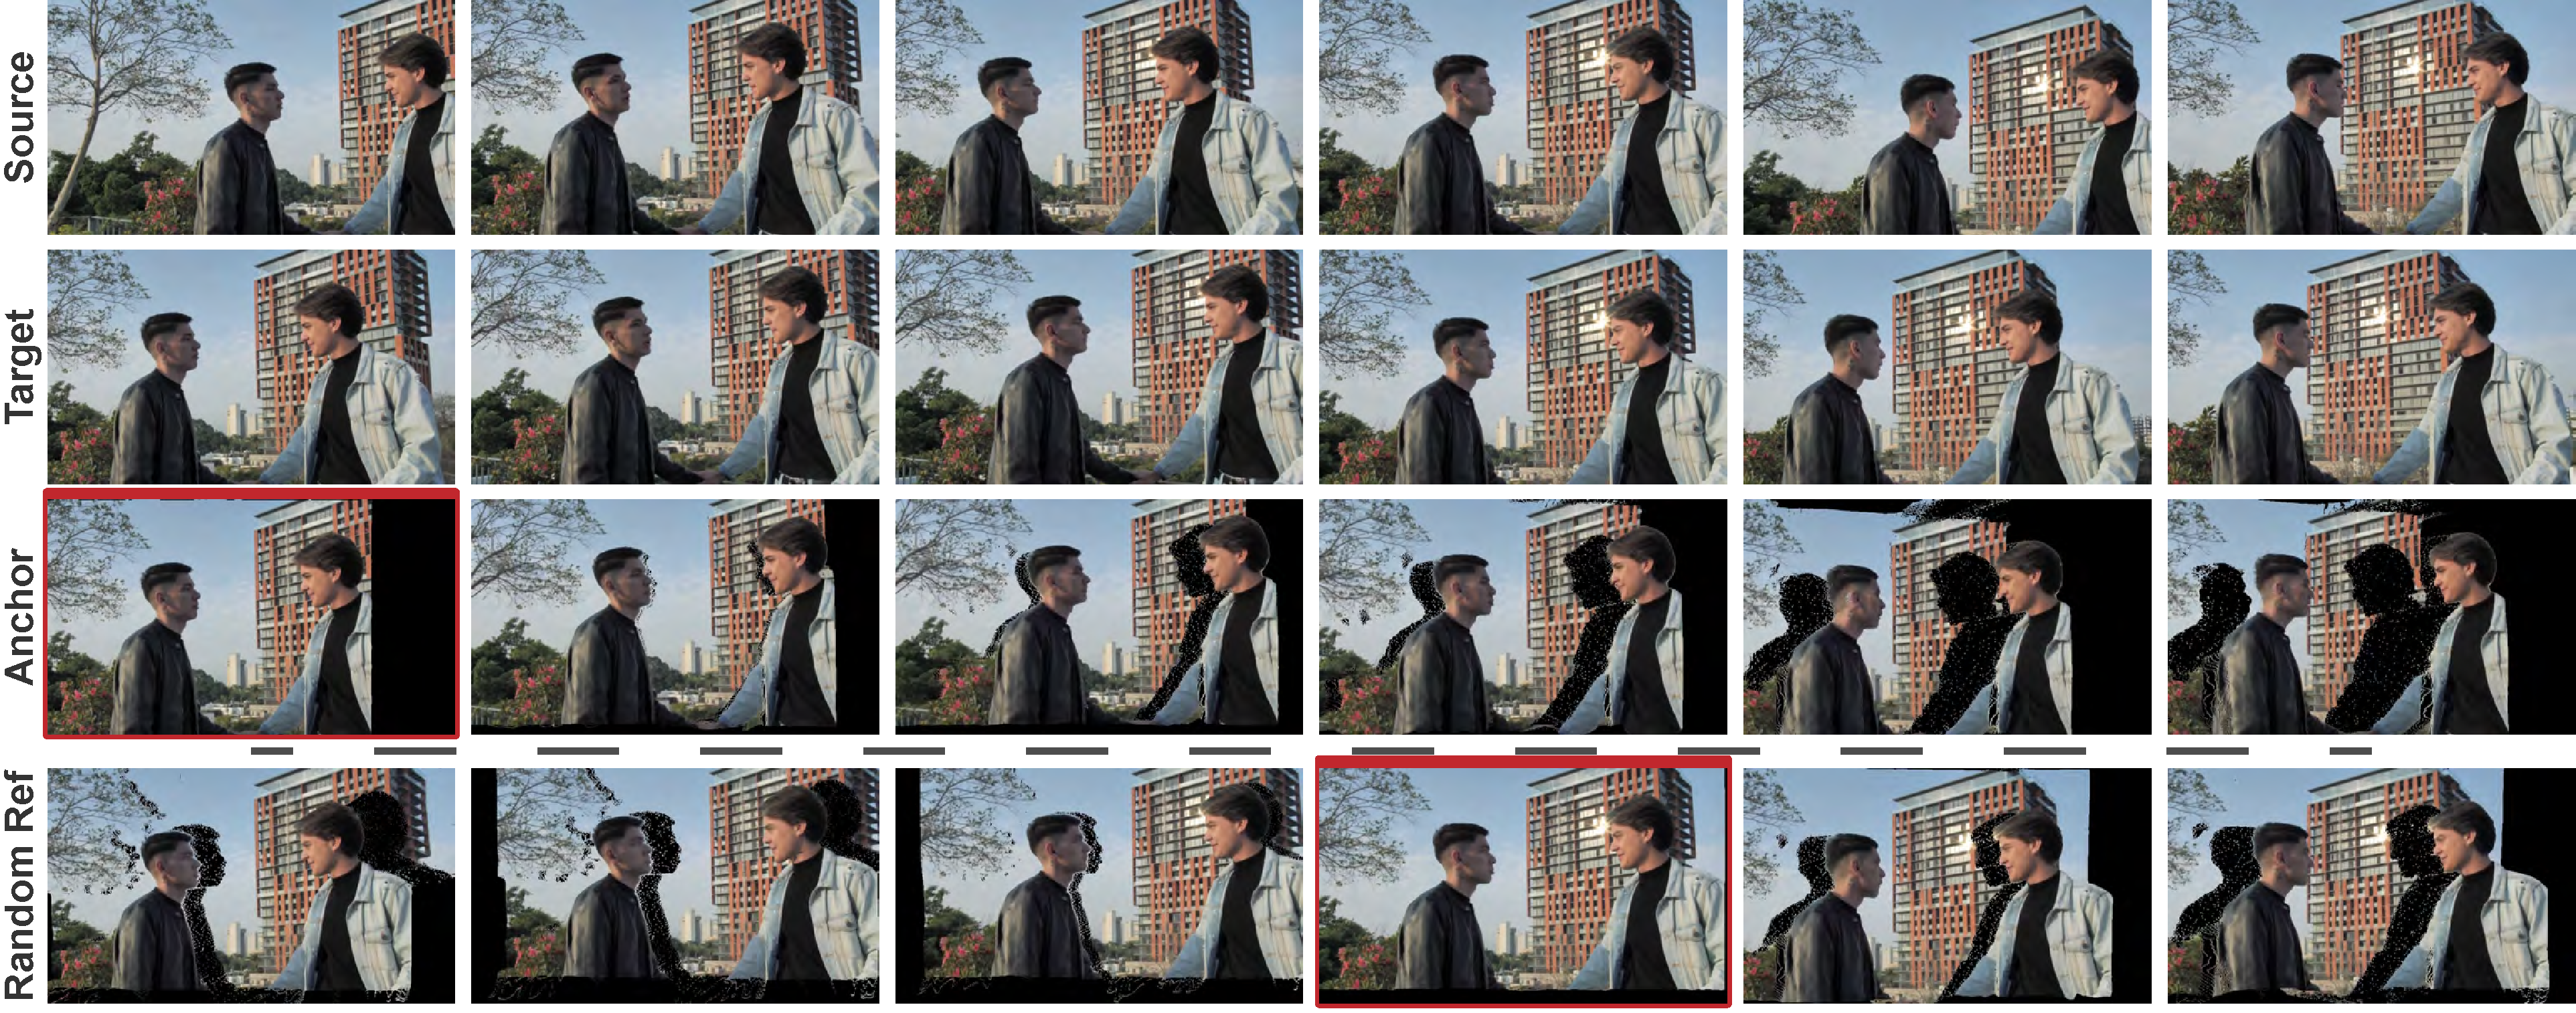
\includegraphics[width=\linewidth]{figures/video_triplets.pdf}
%     \vspace{-0.25in}
%     \caption{
%         \textbf{Our Pseudo Multi-View Triplet and Training Augmentations.}
%         The \textbf{top three rows} illustrate our core training triplet: the \textit{Source Video} ($V_s$), the \textit{Target Video} ($V_t$), and the synthetically generated \textit{Anchor Video} ($V_a$). By default, $V_a$ is created by forward-warping a reference frame from $V_s$ to align with the $V_t$ trajectory. This process can incorporate augmentations such as 3D-aware noise injection (into the $V_s$ reference frame before warping) and flexible reference frame selection, simulating inference-time artifacts and promoting robustness (see Section~\ref{sec:technical_augmentations}).
%         The \textbf{bottom row} shows an example of our Flexible Anchor Reference Frame Warping augmentation. To improve robustness, we can vary the reference frame for warping (e.g., warping from $V_s[40]$ instead of $V_s[0]$ as shown by \red{red bounding boxes}). This variability, made possible by our dense tracking method, forces the model to attend to the anchor's geometric guidance across diverse temporal origins. This augmentation is discussed in Sec.~\ref{sec:results}.
%     }
%     \label{fig:triplets}
%     \vspace{-0.2in}
% \end{figure*}

% The video reshooting task requires synthesizing a high-fidelity \textit{target video}, $V_{t}$, based on a new, desired camera path. At inference time, our model is conditioned on two primary inputs: the \textit{source video} ($V_{s}$), which is the original, high-quality monocular video serving as the "texture and content" reference; and the \textit{anchor video} ($V_{a}$), which defines the target camera motion. This anchor video is typically pre-rendered from a 3D representation (e.g., a sparse point cloud or mesh projection) of the original scene, derived from estimated depth and camera poses for the new trajectory, similar to Figure~\ref{fig:triplets}.

% Following recent approaches~\cite{yu2025trajectorycrafter,ex4d,jeong2025reangle,bai2024syncammaster,wang2025epic}, we utilize an anchor video as a primary conditioning signal. This choice is driven by several factors:
% \begin{description}[noitemsep, topsep=0pt, partopsep=0pt, leftmargin=0pt, style=unboxed, font=\normalfont\bfseries]
%     \item[Intuitive Visual Guidance] An anchor video provides a dense, intuitive visual representation of the desired target camera trajectory, empirically shown to be more effective for guiding generative models than explicit camera poses.
%     \item[Self-Supervised Training Requirement] It is essential for our novel self-supervised training strategy (detailed in Section~\ref{sec:self_supervision}). Since our method generates pseudo-views from 2D crops without modifying underlying 3D camera parameters, conditioning on relative camera poses is not a viable approach. The anchor video instead provides the concrete spatiotemporal target necessary for our pseudo multi-view training pairs.
% \end{description}

% This anchor video, by its nature, is imperfect. It suffers from artifacts such as holes from occlusions, and inaccuracies due to errors in depth and pose estimation. It is therefore unsuitable for direct viewing but is essential for defining the target camera trajectory. While some existing approaches attempt to generate the final video using only $V_{a}$ as input~\cite{ex4d,chen2025reconstruct}, this forces the model to rely entirely on its generative priors to hallucinate all texture, leading to outputs that are inconsistent with the original video's content (see Fig.~\ref{fig:motivation}). The model's core task is therefore to generate a new video $V_{t}$ that faithfully follows the camera motion of $V_{a}$ while replacing its distorted and incomplete content with the clean, temporally consistent texture from $V_{s}$.

% This two-stream input design immediately presents the central challenge of this work: to train this model in a fully supervised manner, we would ideally need a large-scale dataset of triplets $(V_{s}, V_{a}, V_{t})$, where $V_{t}$ is the pristine, real-world ground-truth video corresponding to the $V_{a}$ camera path. However, acquiring such a dataset is logistically intractable at the vast scale and diversity required for robust model training. In the following sections, we describe our novel self-supervised approach that generates precisely this training triplet from monocular videos alone, bypassing this data requirement entirely.

% \subsection{Self-Supervision from Monocular Video}
% \label{sec:self_supervision}

% To address the challenges of data acquisition, we introduce a novel self-supervised strategy that synthesizes the required $(V_s, V_a, V_t)$ training triplets solely from abundant monocular videos.

% \subsubsection{Pseudo-View Triplet Generation}
% \label{sec:pseudo_view_triplet}

% From a single input video $V$, we first employ a smooth video cropper to generate two distinct clips. These clips, which will form our \textit{source video} ($V_s$) and \textit{target video} ($V_t$) for the training triplet, each follow independent \textit{smooth random-walk trajectories} that emulate dynamic camera motion, as shown in Figure~\ref{fig:teaser}. Each trajectory is generated by sampling an adaptive number of random control points within the frame boundaries, with the overall motion magnitude governed by a tunable scale parameter. A \textit{natural cubic spline} is then fitted through these control points to produce a continuous and smooth crop trajectory.

% \begin{figure*}
%     \centering
%     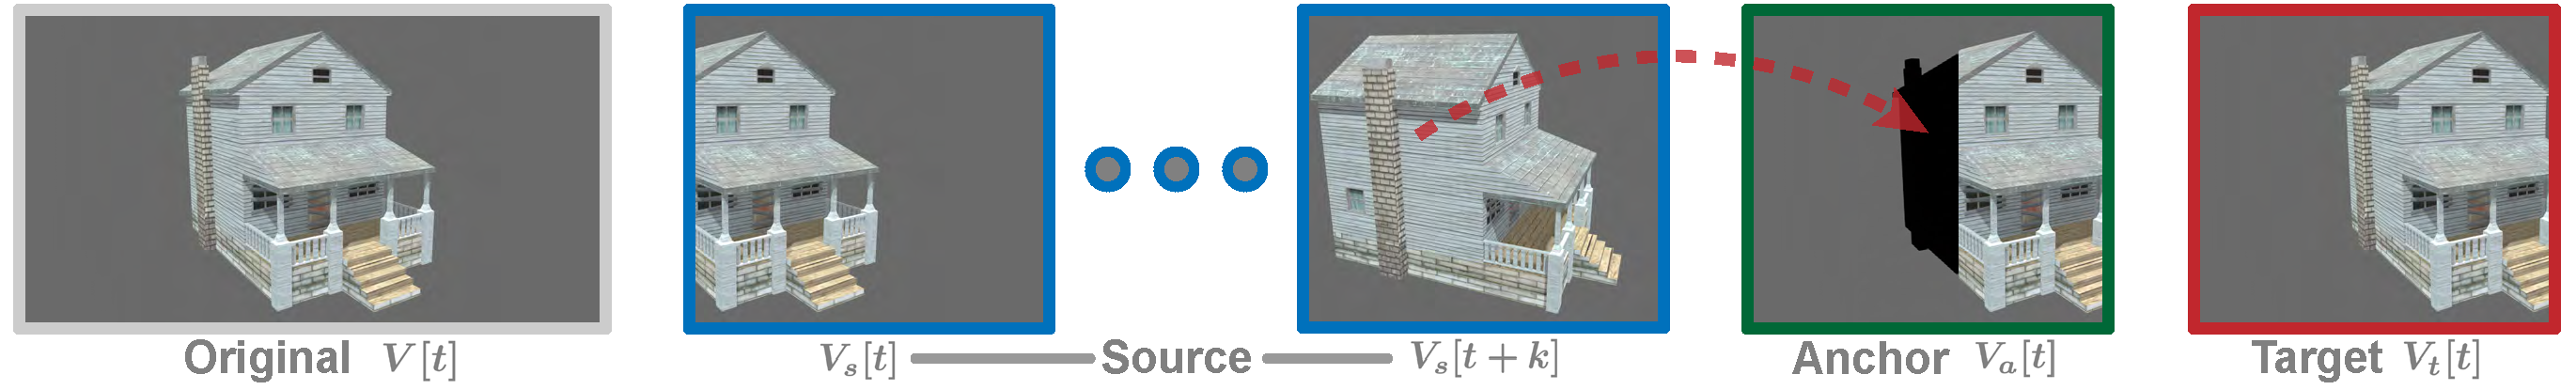
\includegraphics[width=0.8\linewidth]{figures/impl_reprojection.pdf}
%     \vspace{-0.1in}
%     \caption{
%     \textbf{Implicit 3D Reasoning in our Self-Supervised Setup.}
%     Our training method forces the model to learn 3D structure from 2D data.
%     To reconstruct the \textit{Target} $V_t$ at frame $t$, the model is given the disoccluded (holed) \textit{Anchor} $V_a[t]$.
%     The corresponding \textit{Source} frame $V_s[t]$ may not contain the missing texture (e.g., the side of the building).
%     The model is forced to find this texture in a different source frame, $V_s[t+k]$, where it is visible due to $V_s$'s independent camera motion.
%     This operation of sourcing and "stitching" content across different times and pseudo-viewpoints compels the model to learn an implicit 3D understanding of the scene.
%     % \todo{ADD ATTRIBUTION IN FINAL VERSION}
%     }
%     \label{fig:implicit_3d}
%     \vspace{-0.2in}
% \end{figure*}

% We sample two trajectories using different random seeds, resulting in clips $(V_{s}, V_{t})$ that observe different regions of the same video, effectively mimicking time-synchronized distinct moving cameras. Importantly, the original video $V$ may already exhibit its own inherent camera motion; our method naturally inherits and compounds this motion, capturing complex patterns such as orbits, pans, and zooms from in-the-wild footage.

% We designate the two clips as the \textit{Target Video ($V_{t}$)}, the clip to be reconstructed, and the \textit{Source Video ($V_{s}$)}, the high-fidelity texture reference. Based on both clips, we then synthetically generate the \textit{Anchor Video ($V_{a}$)} to complete the training triplet ($V_{s}, V_{a}, V_{t}$), as described next.

% We generate $V_{a}$ by warping the first frame of the source video ($V_{s}[0]$) to align with the target video's trajectory ($V_{t}$). This warping process, illustrated in Figure~\ref{fig:triplets}, is guided by an offset-aware flow field that combines two components: (1) a dense tracking field (capturing 2D pixel motion) and (2) an \textit{crop offset flow} (capturing the change in pseudo-viewpoint). To obtain the dense tracking field, we use AllTracker~\cite{4d_recon_harley2025alltracker} on the original video $V$ \textit{before} cropping. We chose this state-of-the-art tracking method as it is more effective than simple two-frame optical flow for computing correspondences over long temporal distances, as it leverages all intermediate frames. This combined flow is then used to forward-warp $V_{s}[0]$ over time using softmax splatting~\cite{softmax_splatting}:
% \begin{equation}
% V_{a}[t] = \text{SoftSplat}(V_s[0], F_{\text{comb}}(t)),
% \label{eq:anchor_warping}
% \end{equation}
% where $V_a[t]$ is the $t$-th frame of the anchor video, $\text{SoftSplat}$ is the forward warping operator, and $F_{\text{comb}}(t)$ is our combined offset-aware flow field that maps pixels from $V_s[0]$ to the $t$-th frame of the target's coordinate system. The use of forward warping is a deliberate choice, as it effectively simulates the artifacts, occlusions, and dis-occlusions characteristic of the point-cloud-based anchor videos we use at inference.

% \subsubsection{Implicit 3D-Aware Learning}
% \label{sec:implicit_3d_learning}

% This training setup directly forces the model to learn its inference-time task. It must learn to reconstruct the high-quality, dynamic $V_{t}$ by:

% \begin{description}[noitemsep, topsep=0pt, partopsep=0pt, leftmargin=0pt, style=unboxed, font=\normalfont\bfseries]
%     \item[Ignoring Anchor Artifacts] The model learns to treat $V_{a}$ as a geometric guide, not a texture source.
%     \item[Spatial Content Sourcing] The model is forced to find the correct, high-fidelity textures from $V_{s}$. Because $V_{s}$ and $V_{t}$ are not spatially aligned, the model must use its attention mechanism to find content in different spatial regions of the source.
%     \item[Implicit 3D Reasoning] This setup compels the model to reason about 3D structure. As illustrated in Figure~\ref{fig:implicit_3d}, consider the task of reconstructing frame $t$ of the target video, $V_t$. This frame may contain a disoccluded region (e.g., the side of a building) that is not visible in the corresponding source frame $V_s[t]$. However, because the source video $V_s$ has its own independent camera motion, that same side of the building might be visible in a different frame, $V_s[t+k]$. The model is therefore forced to learn to find and source this non-aligned information, effectively "stitching" a view from $V_s[t+k]$ into the disoccluded hole at frame $t$. This operation of finding and re-projecting texture across different viewpoints and times is a form of implicit 3D reasoning.
%     \item[Generative In-painting] For any regions that are not visible in \textit{any} $V_{s}$ frame, the model learns to leverage the generative priors of the base model to plausibly in-paint (or "hallucinate") the missing details.
% \end{description}

% This self-supervised strategy has several key advantages over synthetic or 3D-annotated approaches, primarily in its simplicity and scalability. Our entire data pipeline relies only on a robust 2D dense tracker. This is a significant advantage, as 2D tracking methods are generally more mature and accurate than 3D annotation techniques. This simplicity means our pipeline is domain-agnostic and can be applied to virtually any monocular video. As a result, we can train on a vast and diverse corpus that includes \textit{photorealistic footage, animation, gaming content, and even videos generated by other Gen-AI models}. This exposes our model to a rich variety of both complex visual phenomena (e.g., water splashing, lens flares) and diverse camera motions (e.g., shaky handheld, professional dolly zooms), all without the domain limitations of synthetic generation.

% It is important to note that our training objective does not directly optimize for 3D reconstruction. Rather, the model is compelled to \textit{implicitly learn} 3D reasoning as a necessary sub-task. In order to successfully reconstruct the target video $V_t$ by sourcing content from $V_s$ and following the geometry of $V_a$, the model must learn to handle occlusions and re-project textures across distinct viewpoints and times from the source video to reconstruct the target video, guided by the anchor video. Therefore, 3D re-rendering emerges as a subset of the capabilities our model learns to solve this complex 2D-based task. This full methodology, combining a domain-agnostic pipeline with a generative diffusion base, produces a model that can also plausibly in-paint, hallucinate realistic textures, and robustly handle diverse video styles in a way that pure 3D reconstruction methods cannot.

% \subsection{Model Architecture and Conditioning}
% \label{sec:architecture}

% \begin{figure*}
%     \centering
%     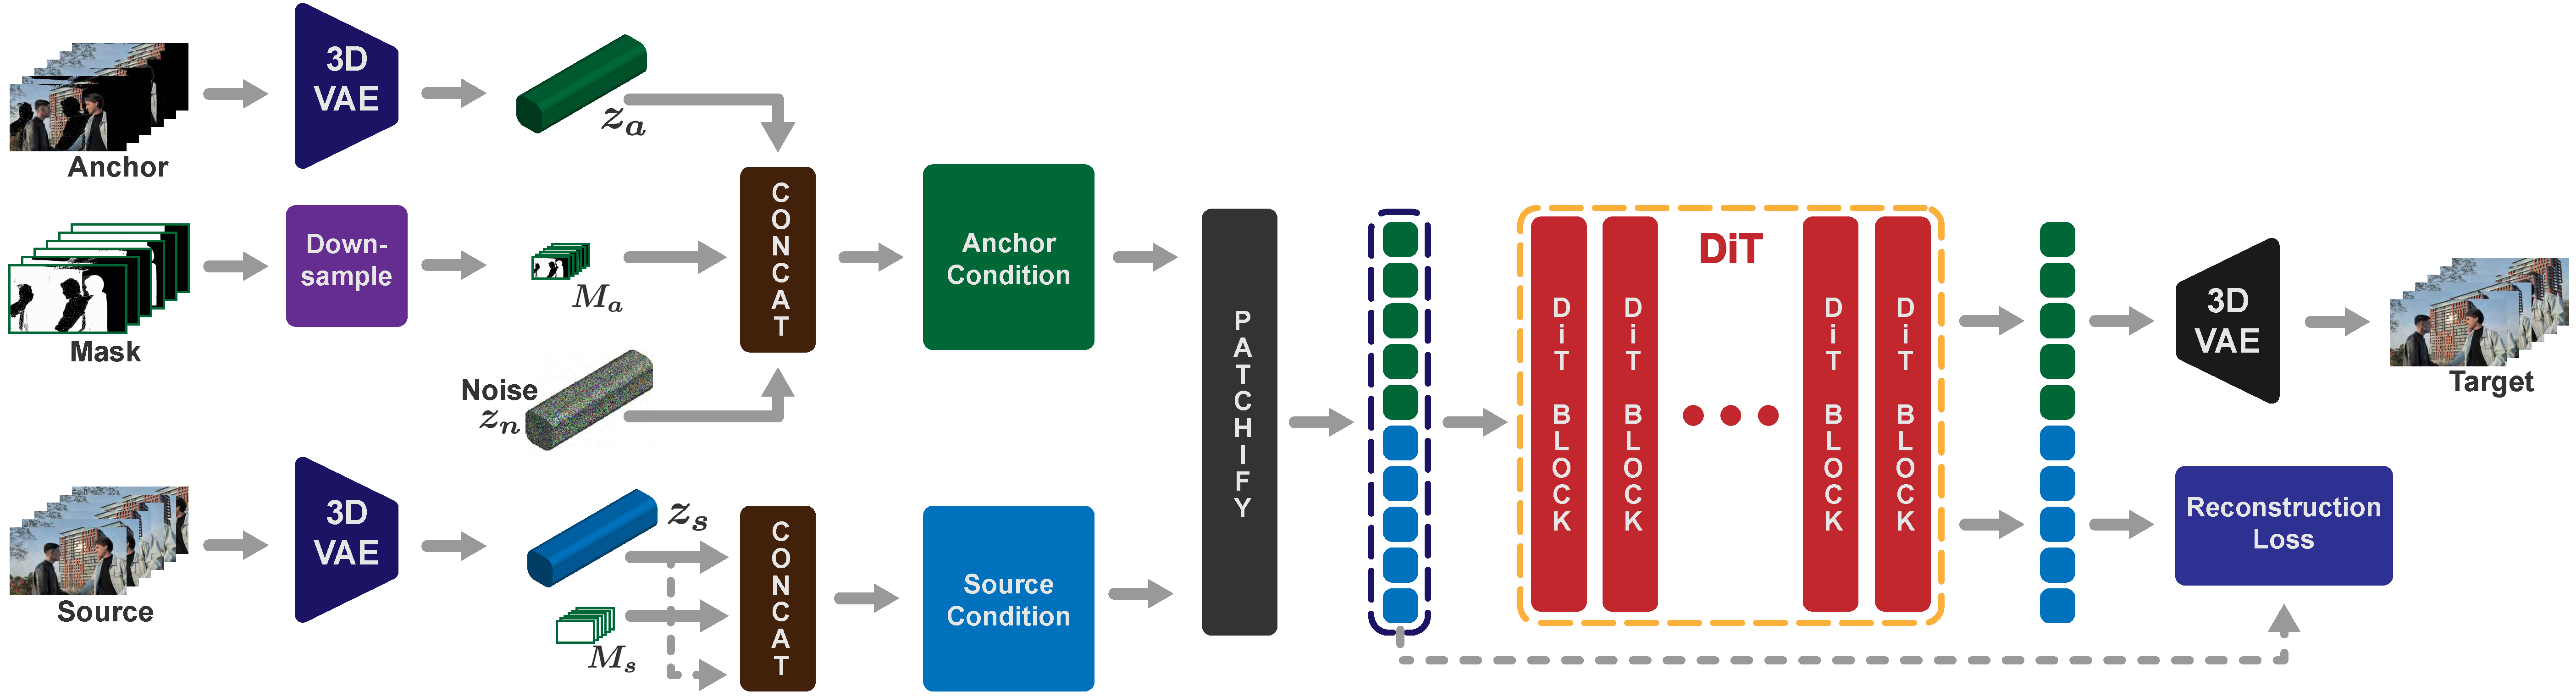
\includegraphics[width=0.8\linewidth]{figures/overview.pdf}
%     \vspace{-0.13in}
%     \caption{\textbf{Overview of our Conditioning Architecture.} Our model adapts a pre-trained DiT-based I2V model~\cite{wan21}. \textbf{(1) VAE Encoding:} The Anchor video ($V_a$) and Source video ($V_s$) are independently encoded into latents by the VAE ($z_a, z_s$). \textbf{(2) Conditioning Setup:} The Anchor latent ($z_a$) is combined with a noise latent ($z_{n}$) and its corresponding mask ($M_a$). The Source latent ($z_s$) is duplicated (replacing $z_{n}$) and combined with an all-ones mask ($M_s$). \textbf{(3) DiT Processing:} The two conditioned streams are temporally concatenated and fed into the DiT blocks. \textbf{(4) Source Token Management \& Denoising:} After each denoising step, the output tokens corresponding to the Source are subjected to an auxiliary reconstruction loss (ensuring content retention).}
%     \label{fig:overview}
%     \vspace{-0.2in}
% \end{figure*}

% Having established our self-supervised training data (Section~\ref{sec:self_supervision}), we now detail the architectural adaptations required to finetune a pre-trained video diffusion model for our task, as illustrated in Figure~\ref{fig:overview}.

% \subsubsection{Video Diffusion Models and DiT Conditioning}
% \label{sec:arch_background}

% Our approach adapts a Diffusion Transformer (DiT) based video model, specifically the WAN 2.2 I2V architecture~\cite{wan21}. DiTs utilize a Transformer architecture for denoising latents, operating as Latent Diffusion Models (LDMs). In essence, the base model is trained to predict the denoised latent from a noisy input, effectively learning to reverse the diffusion process to generate high-quality video frames.

% Conditional signals in DiT architectures can be integrated via: (1) channel concatenation with the noisy latent; (2) dedicated cross-attention layers; or (3) introduction as supplementary tokens processed by the full self-attention mechanism~\cite{bai2025recammaster, peebles2023scalable}. The chosen mechanism is critical for temporal modeling and the application of Rotary Positional Embeddings (RoPE), which encode relative spatiotemporal positional information within transformer blocks, enabling precise understanding of frame order and distance~\cite{bai2025recammaster, su2024roformer}. For our specific adaptations, we leverage a token-based conditioning approach as detailed in the following subsections.

% \subsubsection{Source-Anchor Fusion with Offset RoPE}
% \label{sec:offset_rope}

% Our model is designed to leverage two primary conditions: an anchor video ($V_a$) providing geometric guidance and a source video ($V_s$) offering high-fidelity texture. Integrating $V_s$ as a distinct conditioning signal (e.g., via new cross-attention modules) could typically allow the model to \textit{attend to} $V_s$ frames during the $V_a$ generation process. However, our preliminary experiments, consistent with observations from~\cite{bai2025recammaster}, indicated this strategy is not immediately effective. We found the model struggled to optimize this new data pathway, primarily relying on the $V_a$ input and leading to hallucinated textures inconsistent with the source video. This approach would be computationally expensive and risks perturbing the model's pre-trained weights, thereby degrading its foundational generative capabilities.

% Instead, we adopt the third conditioning strategy: processing both $V_s$ and $V_a$ as tokens within the model's main self-attention mechanism, as detailed in Figure~\ref{fig:overview}. Both the anchor video ($V_a$) and source video ($V_s$) are first independently encoded into latents ($z_a$ and $z_s$ respectively) by the pre-trained VAE.

% The \textit{Anchor condition} is constructed by concatenating its latent ($z_a$) with a noise latent ($z_{n}$) and a downsampled binary mask ($M_a$). This mask specifies regions in $V_a$ lacking valid content, indicating where the model should generate new pixels. The \textit{Source condition} is prepared by duplicating its latent ($z_s$) and concatenating it with an all-ones mask ($M_s$). This ensures the model treats all content in $z_s$ as valid, fully leveraging the source's high-fidelity textures.

% These two prepared conditional streams are then \textit{temporally concatenated} into a single sequence of tokens, which is fed into the DiT blocks. Within the self-attention mechanism of each DiT block, 3D Rotary Positional Embeddings (RoPE) are applied to all tokens. Naively applying continuous RoPE would force the model to learn a fixed relative distance between the source and target frames, thereby limiting generation to a fixed total video length~\cite{bai2025recammaster}. To overcome this, we implement an \textit{Offset RoPE}. We apply a large, fixed offset to the temporal positional embeddings of the $V_s$ tokens only. This effectively decouples the source condition's effective position from the target's, enabling robust, flexible-length video generation at inference time without requiring retraining on varying sequence lengths.

% A crucial aspect of our approach involves managing the source tokens after each denoising step. While the output tokens corresponding to the source video are discarded (as they do not directly contribute to the final $V_t$ generation), it is beneficial to ensure they actively retain meaningful content information from $V_s$. Therefore, during training, we investigate applying a reconstruction loss between the output of the DiT block's source tokens and their original clean VAE latents ($z_s$). This auxiliary loss, discussed further in Section~\ref{sec:implementation_details_or_augmentations}, encourages the source token pathway to preserve the content from the original source video, potentially leading to more effective content sourcing. Only the denoised tokens corresponding to the anchor video are retained and used to compute the primary diffusion loss (Eq.~\ref{eq:diffusion_loss}) during training, or form the input for the subsequent denoising step during inference. This ensures the source tokens serve solely as an internal, context-providing signal within each step, without directly influencing the final output during VAE decoding, while also being actively guided to maintain source content fidelity.

% \subsubsection{Technical Augmentations for Robust Training}
% \label{sec:technical_augmentations}

% Beyond our core architecture, we integrate several technical augmentations to enhance model robustness and generation quality. Detailed configurations are provided in the Supplementary Material.

% \begin{description}[noitemsep, topsep=0pt, partopsep=0pt, leftmargin=0em, style=unboxed, font=\normalfont\bfseries]
%     \item[Source Token Reconstruction Loss] Auxiliary loss applied to ensure content retention from the source video.
%     \item[Adaptive Anchor Mask Background Treatment] We use a high-contrast background (e.g., fluorescent pink) in masked-out regions of the anchor video to improve generation quality, especially in dark scenes.
%     \item[Flexible Anchor Reference Frame Warping] Randomly selecting the reference frame for anchor warping increases robustness to diverse tracking conditions and prevents bias towards early frames.
%     \item[3D-Aware Noise] Gaussian noise is applied to anchor's reference frame before warping, suppressing texture copying from the anchor while preserving its geometric guidance.
% \end{description}

% The detailed implementation of these augmentations is provided in Supplementary.